\documentclass[a4paper]{beamer}%handout


\usepackage{listings}
\usepackage{color}
 
\definecolor{codegreen}{rgb}{0,0.6,0}
\definecolor{codegray}{rgb}{0.5,0.5,0.5}
\definecolor{codepurple}{rgb}{0.58,0,0.82}
\definecolor{backcolour}{rgb}{0.95,0.95,0.92}


%% Add Matlab code
\usepackage{mcode}
%% Add Matlab code end


%% Add watermarks
%\usepackage{draftwatermark}
%% Add watermarks end
\usepackage[utf8]{inputenc}
\usepackage{multicol}
\usepackage{url}
\usepackage{hyperref}
\hypersetup{
	colorlinks=true,
	linkcolor=cyan,          % color of internal links (change box color with linkbordercolor)
    citecolor=green,        % color of links to bibliography
    filecolor=magenta,      % color of file links
    urlcolor=cyan           % color of external links
	}

\graphicspath{{img/}}

\mode<presentation> {

%\usetheme{default}%yes % use %\frametitle in all slides recommended
%\usetheme{AnnArbor}%no
%\usetheme{Antibes} %yes %favorite
%\usetheme{Bergen} %no
%\usetheme{Berkeley} %no
%\usetheme{Berlin} %no
%\usetheme{Boadilla} %yes % good use of paper space
%\usetheme{CambridgeUS} %yes %favorite %use %\frametitle recommended
%\usetheme{Copenhagen}%yes%noframetitle
%\usetheme{Darmstadt}%no
%\usetheme{Dresden}
%\usetheme{Frankfurt}
%\usetheme{Goettingen}
%\usetheme{Hannover}
%\usetheme{Ilmenau}%no
%\usetheme{JuanLesPins}
%\usetheme{Luebeck}
%\usetheme{Madrid}
%\usetheme{Malmoe}
%\usetheme{Marburg}
%\usetheme{Montpellier}
%\usetheme{PaloAlto}
%\usetheme{Pittsburgh}%no
%\usetheme{Rochester}%no
%\usetheme{Singapore}%yees
%\usetheme{Szeged}%no
%\usetheme{Warsaw}%no

% As well as themes, the Beamer class has a number of color themes
% for any slide theme. Uncomment each of these in turn to see how it
% changes the colors of your current slide theme.

%\usecolortheme{albatross}
%\usecolortheme{beaver}
%\usecolortheme{beetle}
%\usecolortheme{crane}
\usecolortheme{dolphin}
%\usecolortheme{dove}
%\usecolortheme{fly}
%\usecolortheme{lily}
%\usecolortheme{orchid}
%\usecolortheme{rose}
%\usecolortheme{seagull}
%\usecolortheme{seahorse}
%\usecolortheme{whale}
%\usecolortheme{wolverine}

\setbeamertemplate{footline} % To remove the footer line in all slides uncomment this line
%\setbeamertemplate{footline}[page number] % To replace the footer line in all slides with a simple slide count uncomment this line

\setbeamertemplate{navigation symbols}{} % To remove the navigation symbols from the bottom of all slides uncomment this line
}

%----------------------------------------------------------------------------------------
%	NEW COMMANDS
%----------------------------------------------------------------------------------------

\newcommand{\Conv}{\mathop{\scalebox{1.5}{\raisebox{-0.2ex}{$\ast$}}}}%
%\linespread{1.3}

%----------------------------------------------------------------------------------------
%	TITLE PAGE
%----------------------------------------------------------------------------------------

\title[Introduction]{Digital Image Processing} % The short title appears at the bottom of every slide, the full title is only on the title page

\author{Prof. Tiago Vieira} % Your name
\institute[UFAL] % Your institution as it will appear on the bottom of every slide, may be shorthand to save space
{
Universidade Federal de Alagoas \\ % Your institution for the title page
\medskip
\textit{tvieira@ic.ufal.br} % Your email address
}
\date{\today} % Date, can be changed to a custom date


%----------------------------------------------------------------------------------------
%	TITLE PAGE
%----------------------------------------------------------------------------------------

\subtitle{Intensity Transformation}

%------------------------------------------------

\begin{document}

%------------------------------------------------

\begin{frame}
\titlepage % Print the title page as the first slide
\end{frame}

%------------------------------------------------

\begin{frame}{Contents}
\setcounter{tocdepth}{1}
\tableofcontents
\end{frame}

%----------------------------------------------------------------------------------------
%	PRESENTATION SLIDES
%----------------------------------------------------------------------------------------

\section{Background}

%----------------------------------------------------------------------------------------
%
%\begin{frame}
%Overview
%\begin{figure}
%\centering
%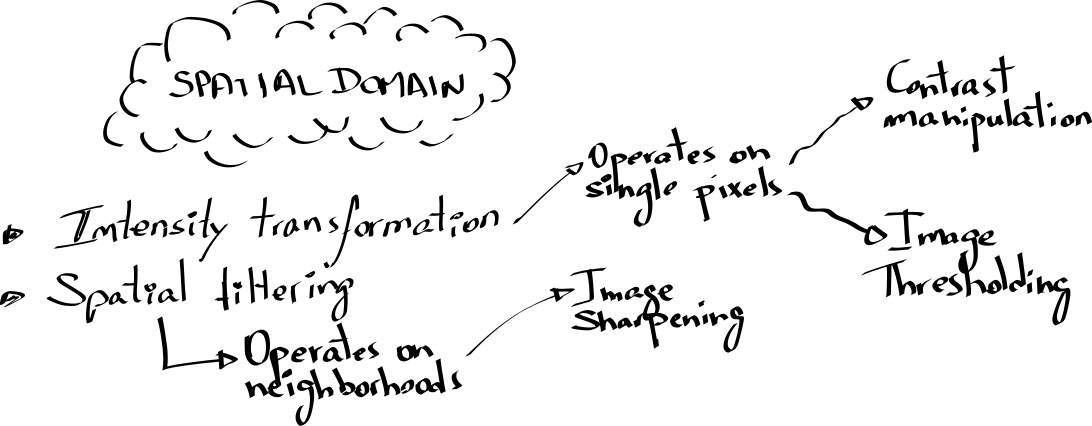
\includegraphics[width=\textwidth]{overview.png}
%\end{figure}
%\end{frame}

%----------------------------------------------------------------------------------------

\begin{frame}
Spatial domain processes can be denoted by
\begin{equation}
g(x,y) = T\left [f(x,y)\right ]
\end{equation}
\begin{itemize}
\item $f(x,y)$ - Input image.
\item $g(x,y)$ - Output image.
\item $T[\cdot]$ - Operator on $f$ defined over a neighborhood of point $(x,y)$.
\end{itemize}
\end{frame}

%----------------------------------------------------------------------------------------

\begin{frame}
Spatial domain processes can be denoted by
\begin{equation}
g(x,y) = T\left [f(x,y)\right ]
\end{equation}
\begin{itemize}
\item Spatial filtering using a $3\times 3$ mask.
\end{itemize}
\begin{figure}
\centering
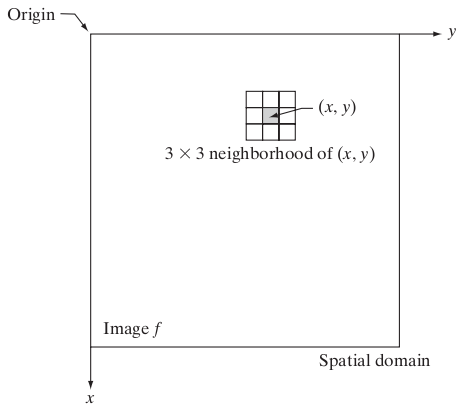
\includegraphics[width=.5\textwidth]{fig-3-1}
\end{figure}
\end{frame}

%----------------------------------------------------------------------------------------

\begin{frame}
\begin{itemize}
\item Smallest neighborhood size $1\times 1$.
\item In this case, we have an \textit{intensity transformation} function
\begin{equation}
s = T(r).
\end{equation}
where $s$ and $r$ denote the intensity of $g$ and $f$ at point $(x,y)$, respectively.
\end{itemize}
\end{frame}

%----------------------------------------------------------------------------------------

\begin{frame}
Examples of contrast stretching and thresholding.
\begin{figure}
\centering
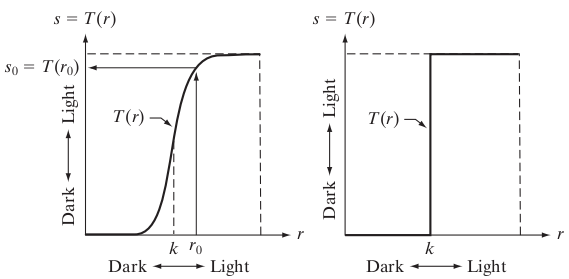
\includegraphics[width=.9\textwidth]{fig-3-2}
\end{figure}
\end{frame}

%----------------------------------------------------------------------------------------

\section{Some basic intensity transformations}

%----------------------------------------------------------------------------------------

\subsection{Image negatives}

%----------------------------------------------------------------------------------------

\begin{frame}
Basic intensity transformations:
\begin{figure}
\centering
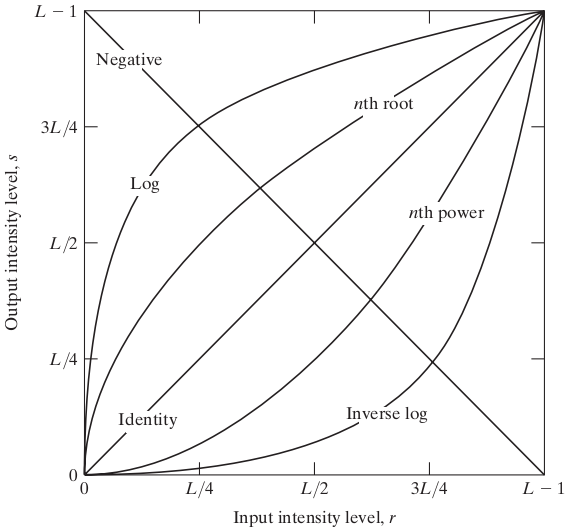
\includegraphics[width=.7\textwidth]{fig-3-3}
\end{figure}
\end{frame}

%----------------------------------------------------------------------------------------

\begin{frame}
\frametitle{Image negative}
\begin{equation}
s = L - 1 - r
\end{equation}
particularly suited for enhancing white or gray detail embedded in dark regions.
\begin{figure}
\centering
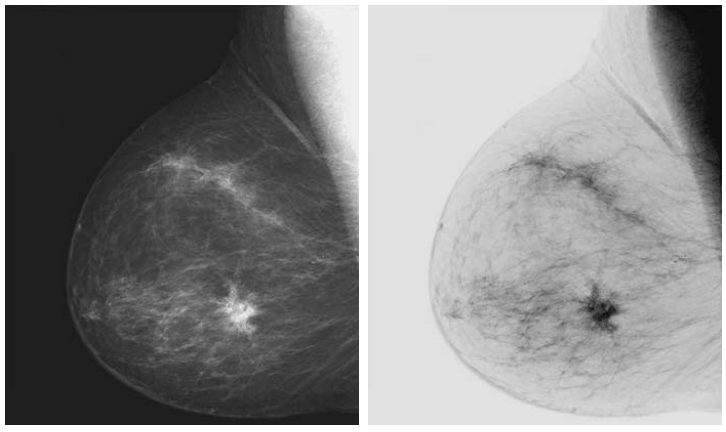
\includegraphics[width=.6\textwidth]{fig-3-4}
\end{figure}
\end{frame}

%----------------------------------------------------------------------------------------

\subsection{Log transformations}

%----------------------------------------------------------------------------------------

\begin{frame}
\frametitle{Log transformations}
\begin{equation}
s=c\log(1+r),
\end{equation}
\begin{itemize}
\item Where $c$ is a constant and it is assumed that $r\geq 0$.
\item The log transform maps a narrow range of low intensity values in the input into a wider range of output levels.
\item Used to expand the dark pixels in an image while compressing the higher-level values.
\item The opposite is true of the inverse log transformation.
\item Compresses the dynamic range of images with large variations in
pixel values. 
\end{itemize}
\end{frame}

%----------------------------------------------------------------------------------------

\begin{frame}
Classical application of the log transform; Fourier Spectra:
\begin{itemize}
\item It has values typically within range $\in[0,10^{6}]$ or higher.
\item Such wide range cannot be faithfully represented without the aid of a transform:
\end{itemize} 
\begin{figure}
\centering
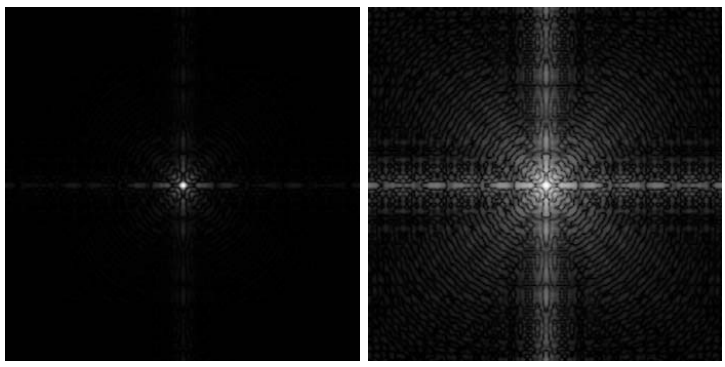
\includegraphics[width=
\textwidth]{fig-3-5}
\end{figure}\end{frame}

%----------------------------------------------------------------------------------------

\subsection{Power-lay (gamma) transformations}

%----------------------------------------------------------------------------------------

\begin{frame}{Power-lay (gamma) transformation}
Basic form:
\begin{equation}
s = cr^{\gamma},
\end{equation}
where $c$ and $\gamma$ are positive constants.
\begin{figure}
\centering
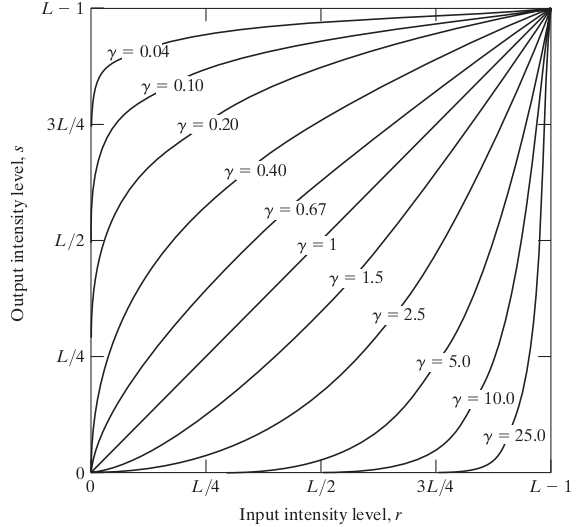
\includegraphics[width=.6\textwidth]{fig-3-6}
\end{figure}
\end{frame}

%----------------------------------------------------------------------------------------

\begin{frame}
Gamma correction.
\begin{itemize}
\item Cathode Ray Tube (CRT) have intensity-to-voltage response that is a power function (exponents $\in[1.8,2.5]$.
\item Example of gamma-correction using $s=r^{1/2.5}=r^{0.4}$:
\end{itemize}
\begin{figure}
\centering
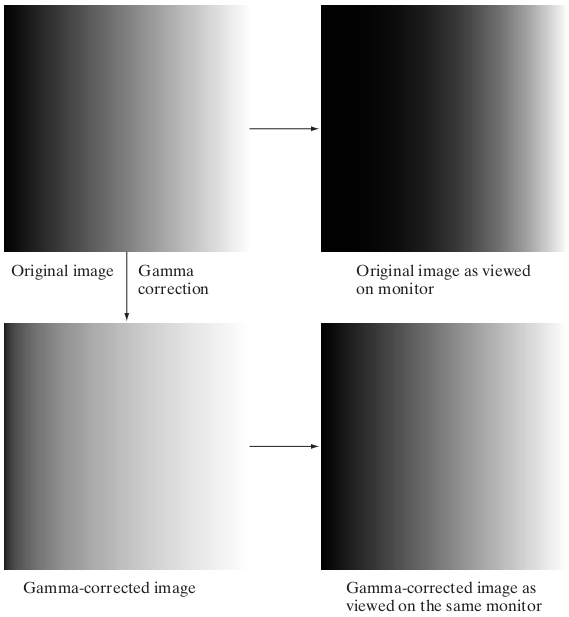
\includegraphics[width=.5\textwidth]{fig-3-7}
\end{figure}
\end{frame}

%----------------------------------------------------------------------------------------

\begin{frame}
Gamma correction is important:
\begin{itemize}
\item Accurately display an image in a computer screen.
\item An image shown in a website is seen by millions of different screens.
\item Varying gamma affects color.
\end{itemize}
\end{frame}

%----------------------------------------------------------------------------------------

\begin{frame}
\begin{figure}
\centering
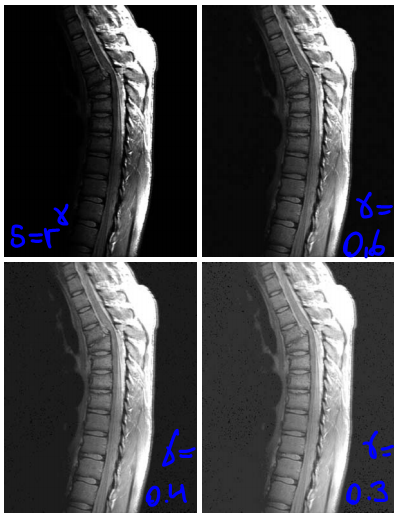
\includegraphics[width=.5\textwidth]{fig-3-8-2}
\end{figure}
\end{frame}

%----------------------------------------------------------------------------------------

\begin{frame}
\begin{figure}
\centering
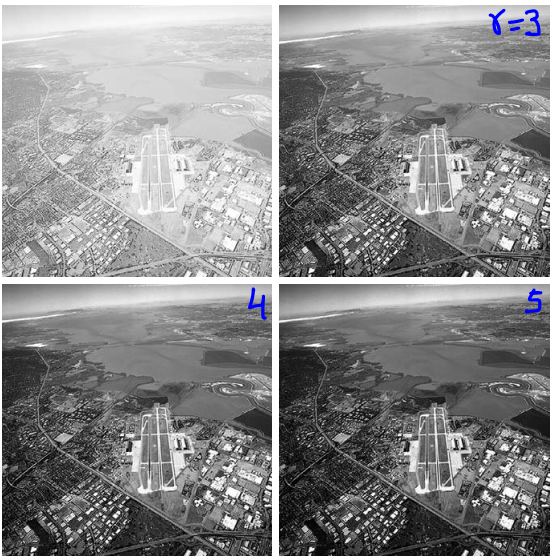
\includegraphics[width=.75\textwidth]{fig-3-9}
\end{figure}
\end{frame}

%----------------------------------------------------------------------------------------

\subsection{Piecewise-Linear Transformation Functions}

%----------------------------------------------------------------------------------------

\begin{frame}{Piecewise-Linear Transformation Functions}
\begin{itemize}
\item Piece-wise linear functions can be arbitrarily complex.
\item Require, however, considerably more user input.
\end{itemize}
\end{frame}

%----------------------------------------------------------------------------------------

\subsubsection{Contrast stretching}

%----------------------------------------------------------------------------------------

\begin{frame}{Contrast stretching}
Low-contrast images can result from;
\begin{itemize}
\item poor illumination;
\item lack of dynamic range in the imaging sensor, or even a;
\item wrong setting of a lens aperture
during image acquisition.
\end{itemize}
\begin{block}{Contrast stretching}
Process that expands the range of intensity levels in an image so that it spans the full intensity range of the recording medium or display device.
\end{block}
\end{frame}

%----------------------------------------------------------------------------------------

\begin{frame}
Picewise-linear transformation.
\begin{columns}
\begin{column}{.5\textwidth}
\begin{itemize}
\item $r_{1} = s_{1}$ and $r_{2} = s_{2} \rightarrow$ linear transformation, i. e., no change.
\item $r_{1} = r_{2}$, $s_{1} = 0$ and $s_{2} = L-1 \rightarrow$ \textit{thresholding}.
\item In general, $r_{1} \leq r_{2}$ and $s_{1} \leq s_{2}$, preserving the order of intensity levels and preventing the creation of intensity artifacts.
\end{itemize}
\end{column}
\begin{column}{.5\textwidth}
\begin{figure}
\centering
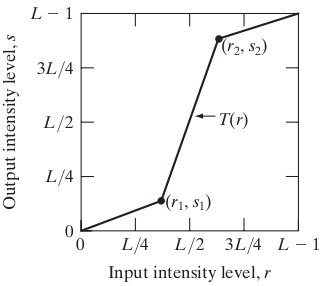
\includegraphics[width=\textwidth]{fig-3-10a}
\end{figure}
\end{column}
\end{columns}
\end{frame}

%----------------------------------------------------------------------------------------

\begin{frame}
Scanning electron microscope image of pollen $\times 700$.
\begin{enumerate}
\item $(r_{1},s_{1}) = (r_{min},0)$ and $(r_{2}, s_{2}) = (r_{max}, L-1)$.
\item $(r_{1},s_{1}) = (m,0)$ and $(r_{2}, s_{2}) = (m, L-1)$.
\end{enumerate}
\begin{figure}
\centering
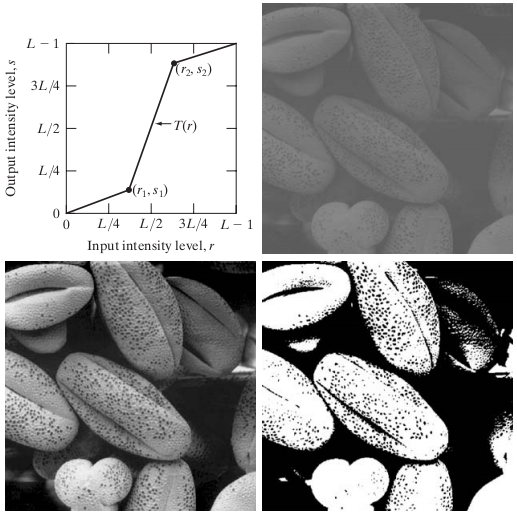
\includegraphics[width=.55
\textwidth]{fig-3-10}
\end{figure}\end{frame}

%----------------------------------------------------------------------------------------

\subsubsection{Intensity-level slicing}

%----------------------------------------------------------------------------------------

\begin{frame}{Intensity-level slicing}
Highlight specific ranges of intensity;
\begin{enumerate}
\item binarize range of interest, or;
\item brightens (or darkens) desired range leaving the rest unchanged.
\end{enumerate}
\begin{figure}
\centering
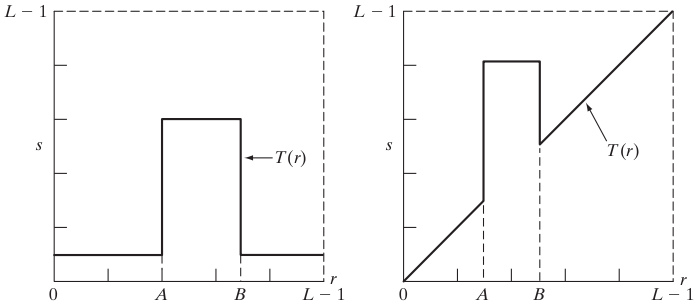
\includegraphics[width=.8\textwidth]{fig-3-11}
\end{figure}
\end{frame}

%----------------------------------------------------------------------------------------

\begin{frame}
Aortic angiogram near the kidney area.
\begin{figure}
\centering
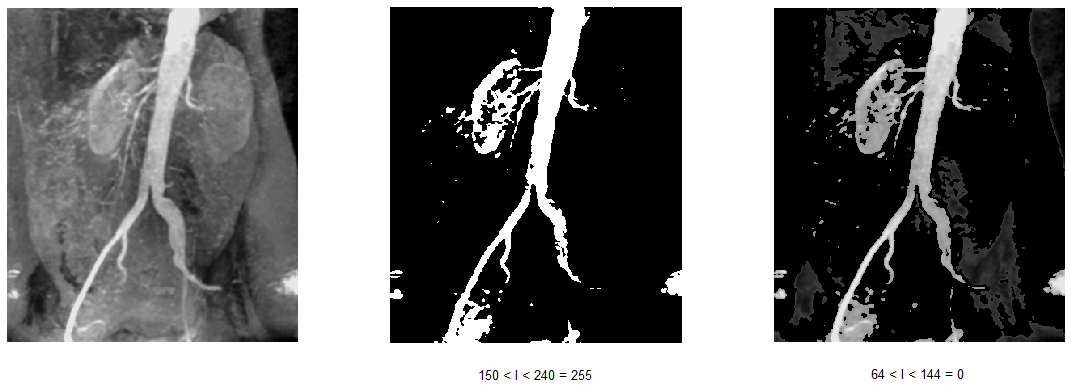
\includegraphics[width=1\textwidth]{fig-3-12b}
\end{figure}
\end{frame}

%----------------------------------------------------------------------------------------

\subsubsection{Bit-plane slicing}

%----------------------------------------------------------------------------------------

%\begin{frame}
%asdf
%%\begin{lstlisting}
%%cdef
%%\end{lstlisting}
%\end{frame}

%----------------------------------------------------------------------------------------

\begin{frame}{Bit-plane slicing}
Highlight the contribution made to total image appearance by specific bits.
\begin{figure}
\centering
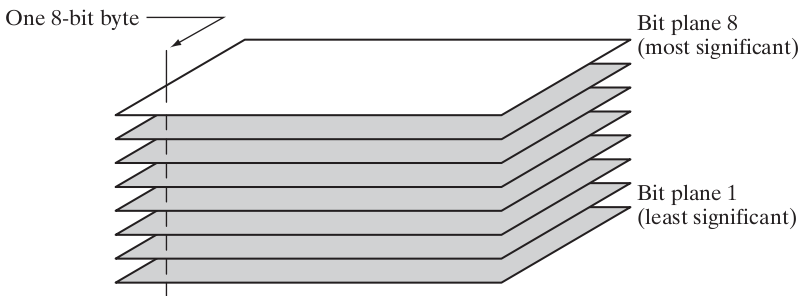
\includegraphics[width=\textwidth]{fig-3-13}
\end{figure}
\end{frame}

%----------------------------------------------------------------------------------------

\begin{frame}
\begin{figure}
\centering
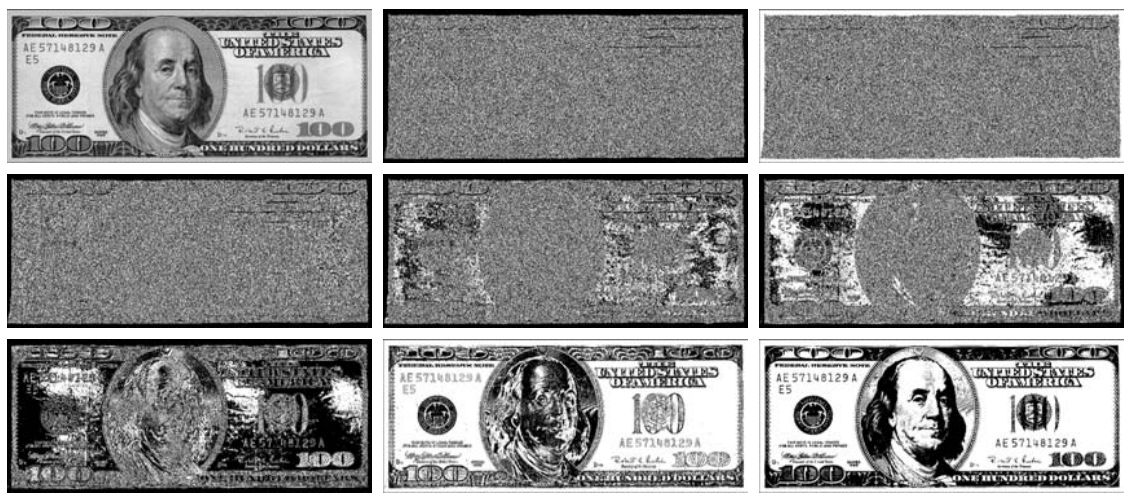
\includegraphics[width=\textwidth]{fig-3-14}
\end{figure}
\end{frame}

%----------------------------------------------------------------------------------------

\begin{frame}
An example application of bit slicing: Image compression:
\begin{figure}
\centering
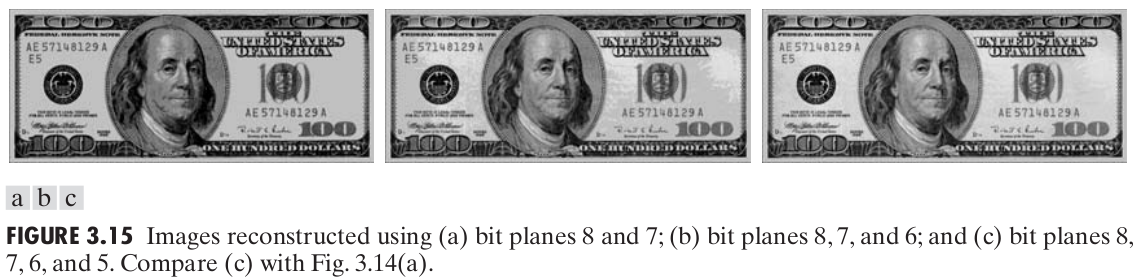
\includegraphics[width=\textwidth]{fig-3-15}
\end{figure}
\begin{itemize}
\item Notice that the 4 most significant bits are sufficient to reasonably ``reconstruct'' the original image (a reduction of 50\% in bit memory storage);
\end{itemize}
\end{frame}

%----------------------------------------------------------------------------------------

\section{Histogram processing}

%----------------------------------------------------------------------------------------

\begin{frame}
\frametitle{Histogram processing}
\begin{itemize}
\item The histogram of a digital image with intensity levels in the range $[0,L-1]$ is a discrete function $h(r_{k}) = n_{k}$ where $r_{k}$ is the $k$th intensity value and $n_{k}$ is the number of pixels in the image with intensity $r_{k}$.
\item The histogram is commonly normalized by $1/n$, with $n=MN$.
\item The probability of occurrence of intensity value $r_{k}$ is $p(r_{k}) = n_{k}/n$, for $k = 0,\ldots,L-1$.
\end{itemize}
\end{frame}

%----------------------------------------------------------------------------------------

\begin{frame}
Examples:
\begin{columns}
\begin{column}{.5\textwidth}
\begin{figure}
\centering
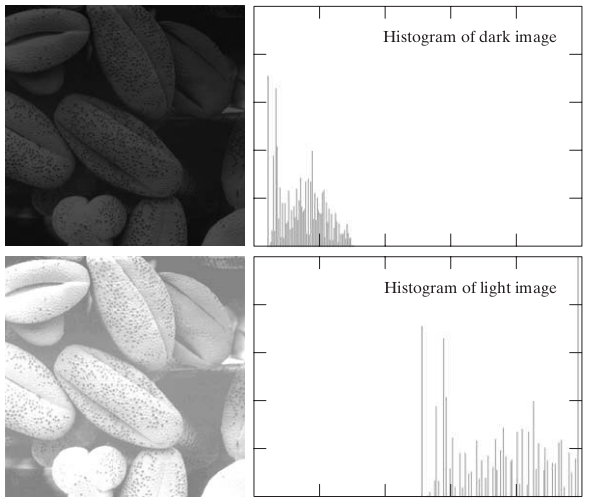
\includegraphics[width=\textwidth]{fig-3-16a}
\end{figure}
\end{column}
\begin{column}{.5\textwidth}
\begin{figure}
\centering
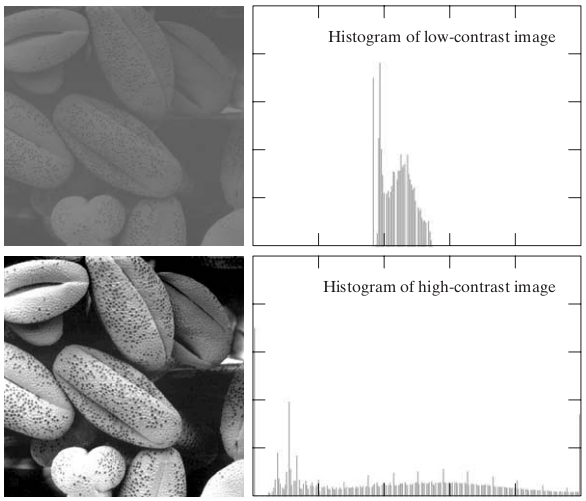
\includegraphics[width=\textwidth]{fig-3-16b}
\end{figure}
\end{column}
\end{columns}
\end{frame}

%----------------------------------------------------------------------------------------

\begin{frame}
Histogram is an important tool for image processing. It is used in
\begin{itemize}
\item Image enhancement.
\item Statistical processing.
\item Compression.
\item Segmentation.
\end{itemize}
Furthermore:
\begin{itemize}
\item It is simple to compute.
\item Cheap hardware implementation.
\item Automatic.
\end{itemize}
\end{frame}

%----------------------------------------------------------------------------------------

\subsection{Histogram equalization}

%----------------------------------------------------------------------------------------

\begin{frame}
\frametitle{Histogram equalization}
\begin{itemize}
\item Consider (momentarily) continuous intensity values.
\item $r\in [0,L-1]$ denotes the intensities of an image to be processed.
\item Consider intensity mappings of the form
\begin{equation}
s=T(r)\ \ 0\leq r \leq L-1.
\end{equation}
\end{itemize}
\end{frame}

%----------------------------------------------------------------------------------------

\begin{frame}
\begin{columns}
\begin{column}{.5\textwidth}
Assume:
\begin{enumerate}
\item $T(r)$ is monotonically increasing in the interval $0\leq r \leq L-1$, and;
\item $0\leq T(r) \leq L-1$ for $0\leq r \leq L-1$.
\end{enumerate}
Considering the inverse
\begin{equation}
r = T^{-1}(s)
\end{equation}
\end{column}
\begin{column}{.5\textwidth}
\begin{figure}
\centering
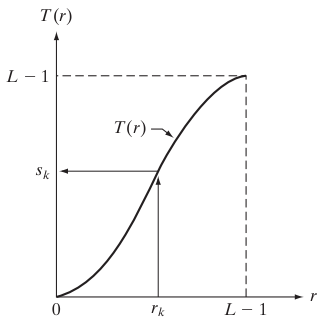
\includegraphics[width=\textwidth]{fig-3-17b}
\end{figure}
\end{column}
\end{columns}
\end{frame}

%----------------------------------------------------------------------------------------

\begin{frame}
\begin{itemize}
\item Intensity levels in an image may be viewed as random variables in the interval $[0,L-1]$.
\item Let $p_{r}(r)$ and $p_{s}(s)$ denote the Probability Density Functions (PDFs) of $r$ and $s$.
\item From probability
theory, if $p_{r}(r)$ and $T(r)$ are known, and $T(r)$ is continuous and differentiable over the range of values of interest, then the PDF of the transformed variable $s$ can be obtained using
\begin{equation}
p_{s}(s) = p_{r}(r) \left |\dfrac{dr}{ds} \right |.
\end{equation}
\end{itemize}
\end{frame}

%----------------------------------------------------------------------------------------

\begin{frame}
Consider the transformation function
\begin{equation}
s = T(r) = \left (L - 1\right ) \int_{0}^{r} p_{r}(w) dw,
\end{equation}
which is the Cumulative Distribution Function (CDF) of random variable $r$, which satisfies previous conditions.

From previous equation, one can derive
\begin{equation}
\dfrac{ds}{dr} = (L-1) \dfrac{d}{dr} \left [ \int_{0}^{r} p_{r}(w) dw \right ] = (L-1)p_{r}(r).
\end{equation}
Substituting this result in $p_{s}(s) = p_{r}(r) \left |\dfrac{dr}{ds} \right |$ yields$\ldots$
\end{frame}

%----------------------------------------------------------------------------------------

\begin{frame}
\[
p_{s}(s) = p_{r}(r) \left |\dfrac{dr}{ds} \right |
\]
\[
p_{r}(r) \left |\dfrac{1}{(L-1)p_{r}(r)} \right |
\]
\begin{equation}
\boxed{p_{s}(s) = \dfrac{1}{L-1}},\ \ 0 \leq s \leq L-1.
\end{equation}
which is a \textit{uniform} probability density function.
\end{frame}

%----------------------------------------------------------------------------------------

\begin{frame}
In other words, using the transformation
\[
\boxed{s = T(r) = \left (L - 1\right ) \int_{0}^{r} p_{r}(w) dw},
\]
yields a random variable $s$ characterized by a uniform PDF.

Note that:
\begin{itemize}
\item $T(r)$ depends on $p_{r}(r)$, but;
\item the resulting $p_{s}(s)$ is \textit{always} uniform, independently of $p_{r}(r)$.
\end{itemize}
\begin{figure}
\centering
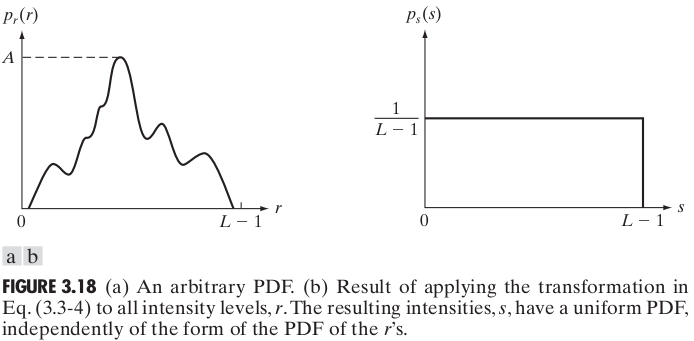
\includegraphics[width=.7\textwidth]{fig-3-18}
\end{figure}
\end{frame}

%----------------------------------------------------------------------------------------

\begin{frame}
\[
p_{r}(r_{k}) = \dfrac{n_{k}}{n},\ \ k = 0,1,\ldots,L-1.
\]
\[
s_{k} = T(r_{k}) = (L-1)\sum_{j=0}^{k}p_{r}(r_{j}).
\]
\begin{equation}
\boxed{s_{k} = \dfrac{(L-1)}{n}\sum_{j=0}^{k}n_{j}},\ \ \ k = 0,1,\ldots,L-1.
\label{eq:histeq}
\end{equation}
where
\[
n = MN
\]
Each input intensity $r_{k}$ is mapped into a level $s_{k}$ in the output image, using Eq.~(\ref{eq:histeq}).
\end{frame}

%----------------------------------------------------------------------------------------

\begin{frame}
Example: Hypothetical $64\times 64 = 4096$ image with $L=8$ intensity levels.
\begin{table}
\centering
\begin{tabular}{ccccc}
\hline
$r_{k}$ & $n_{k}$ & $n_{k}/n$ & $s_{k}$ & $s_{k}$ \\
\hline
0 & 790 & 0.19 & 1.35 & 1 \\
1 & 1023 & 0.25 & 3.10 & 3 \\
2 & 850 & 0.21 & 4.55 & 5 \\
3 & 656 & 0.16 & 5.67 & 6 \\
4 & 329 & 0.08 & 6.23 & 6 \\
5 & 245 & 0.06 & 6.65 & 7 \\
6 & 122 & 0.03 & 6.86 & 7 \\
7 & 81 & 0.02 & 7.00 & 7 \\
\hline
\end{tabular}
\end{table}
\end{frame}

%----------------------------------------------------------------------------------------

\begin{frame}
Illustration of histogram equalization:
\begin{figure}
\centering
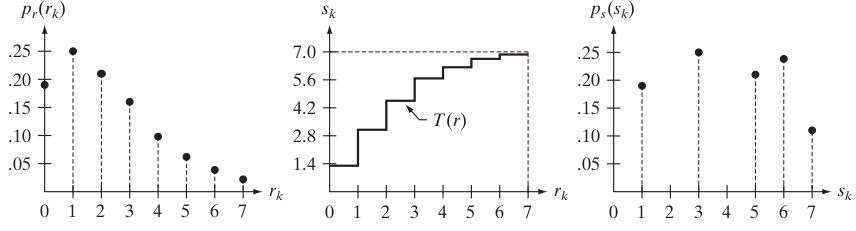
\includegraphics[width=\textwidth]{histeq-1}
\caption{Illustration of histogram equalization of a 3-bit (8 intensity levels) image. (left) Original
histogram. (middle) Transformation function. (right) Equalized histogram.}
\end{figure}
\end{frame}

%----------------------------------------------------------------------------------------

\begin{frame}
Step-by-step histogram equalization:
\begin{enumerate}
\item Compute image's probabilities $p_{r}(r_{k}) = n_{k}/n$.
\item Compute cumulative probability distribution $s_{k} = \left [\left (L-1 \right )/n\right ]\sum_{j=0}^{k}n_{j}$.
\item Map pixels with values $r_{k}$ to intensity values ($s_{k}$).
\end{enumerate}
\begin{block}{Notice}
Histogram equalization has the tendency to wider the range of the intensity values, enhancing the contrast.
\end{block}
\end{frame}

%----------------------------------------------------------------------------------------

\begin{frame}
\begin{figure}[!h]
\centering
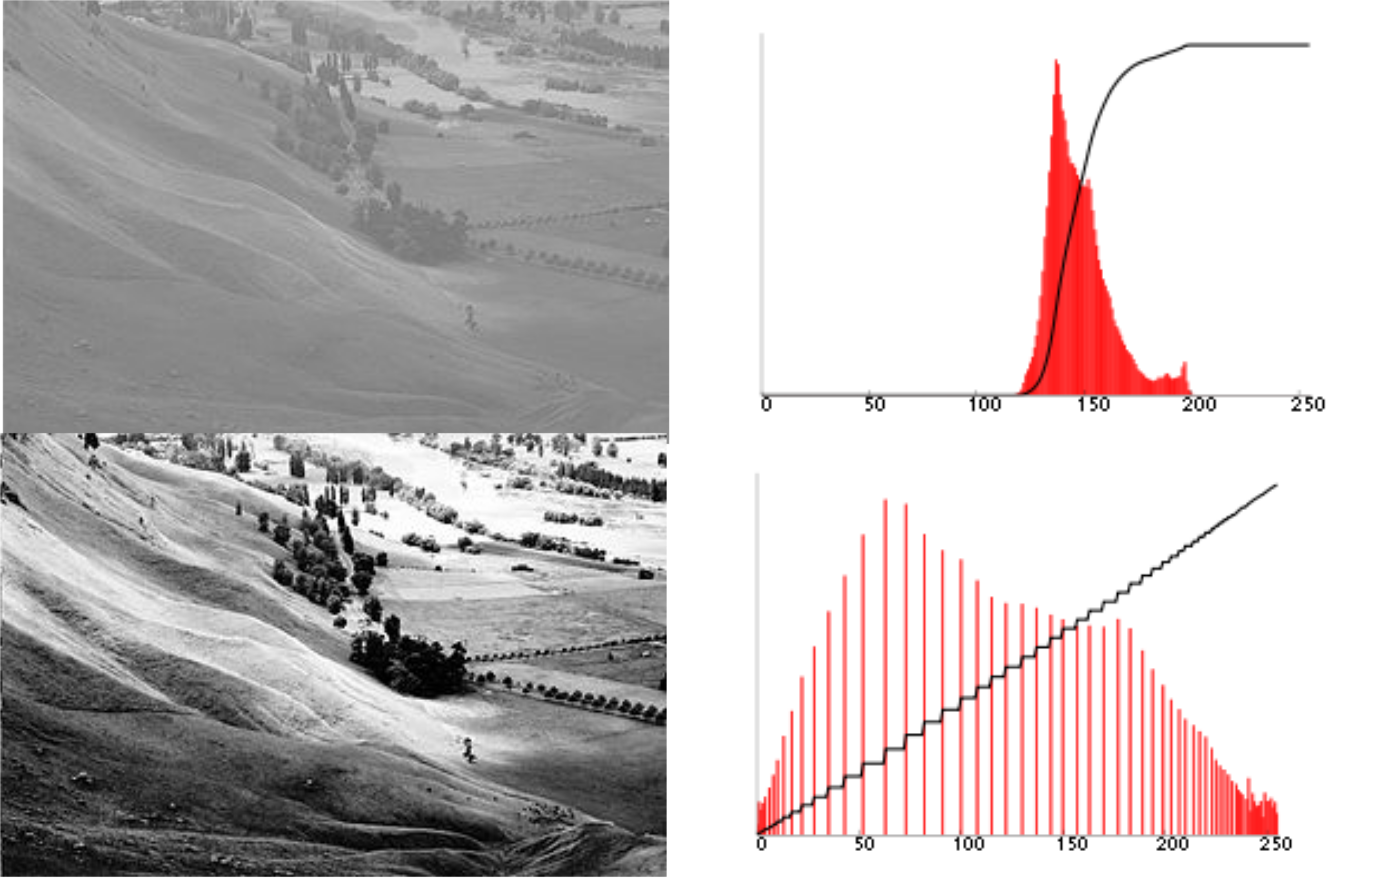
\includegraphics[width=\textwidth]{ex}
\end{figure}
\end{frame}

%----------------------------------------------------------------------------------------

\begin{frame}
\begin{figure}
\centering
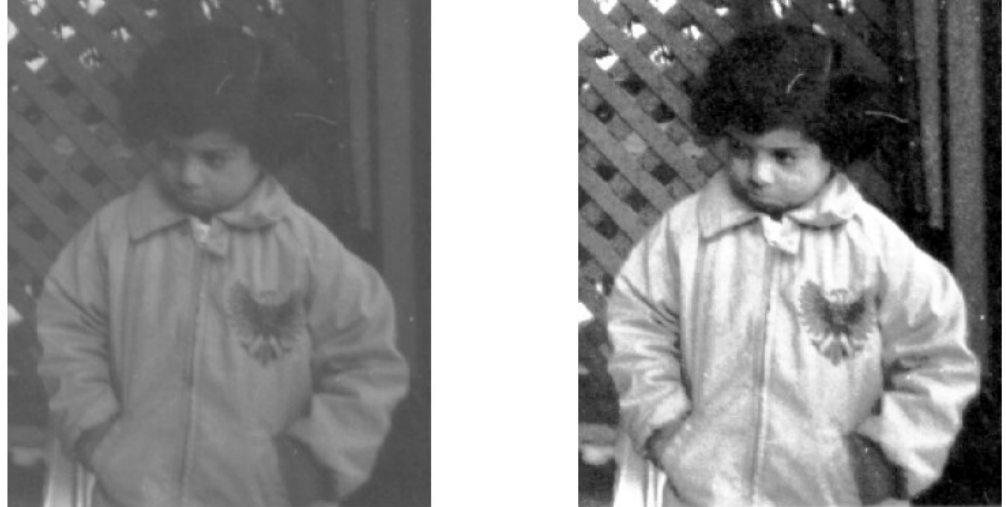
\includegraphics[width=\textwidth]{histeq-2}
\caption{Original (left) and histogram equalized image (right).}
\end{figure}
\end{frame}

%----------------------------------------------------------------------------------------

\begin{frame}
\begin{figure}
\centering
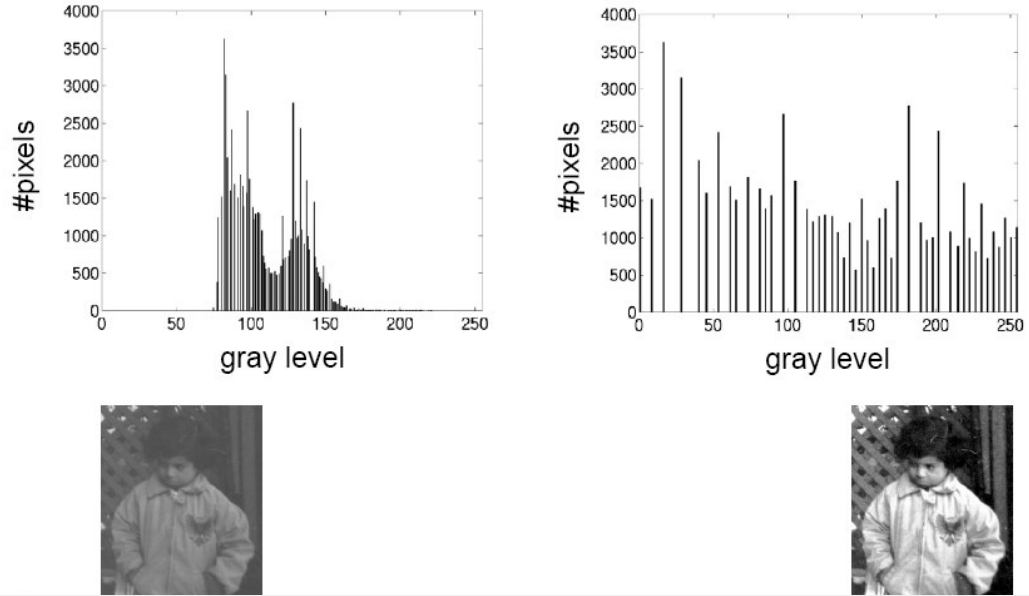
\includegraphics[width=\textwidth]{histeq-3}
\end{figure}
\end{frame}

%----------------------------------------------------------------------------------------

\begin{frame}
\begin{figure}
\centering
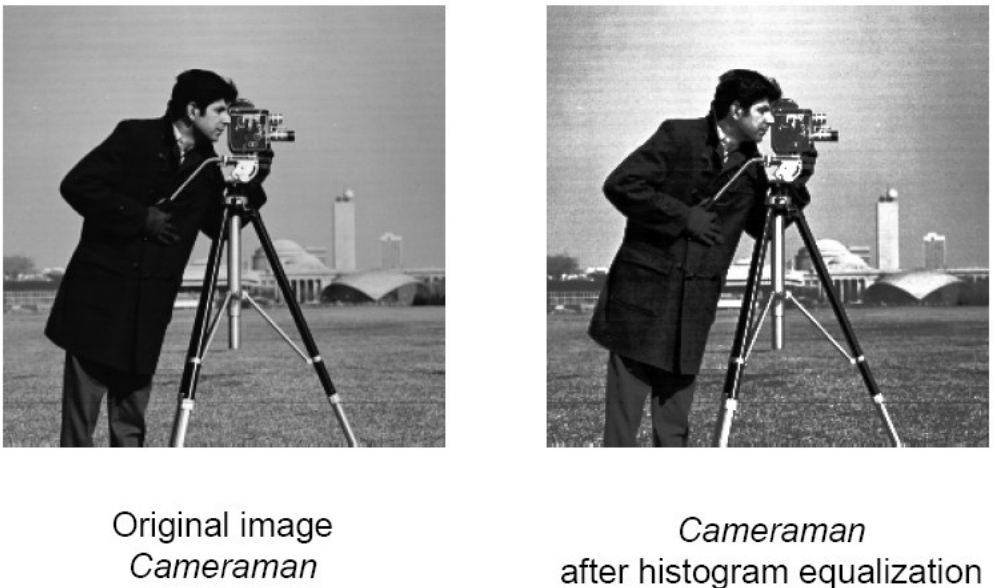
\includegraphics[width=\textwidth]{histeq-4}
\end{figure}
\end{frame}

%----------------------------------------------------------------------------------------

\begin{frame}
\begin{figure}
\centering
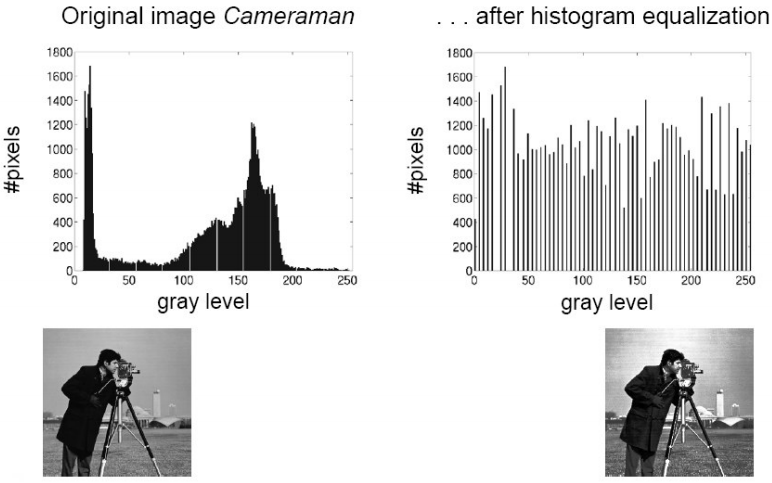
\includegraphics[width=\textwidth]{histeq-5}
\end{figure}
\end{frame}

%----------------------------------------------------------------------------------------

\begin{frame}
\begin{columns}
\begin{column}{.5\textwidth}
\begin{figure}
\centering
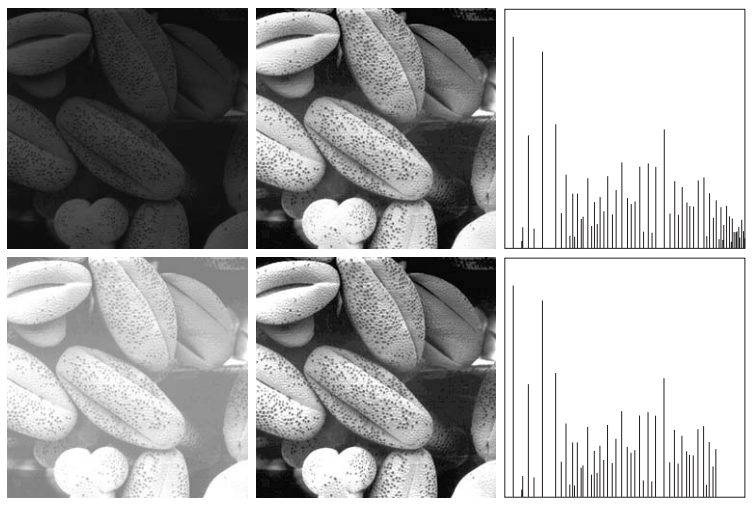
\includegraphics[width=\textwidth]{graos-1}
\end{figure}
\begin{figure}
\centering
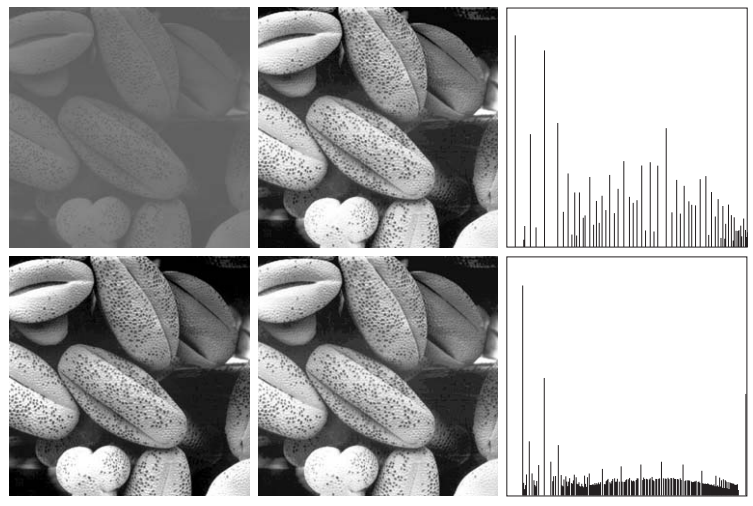
\includegraphics[width=\textwidth]{graos-2}
\end{figure}
\end{column}
\begin{column}{.5\textwidth}
\begin{figure}
\centering
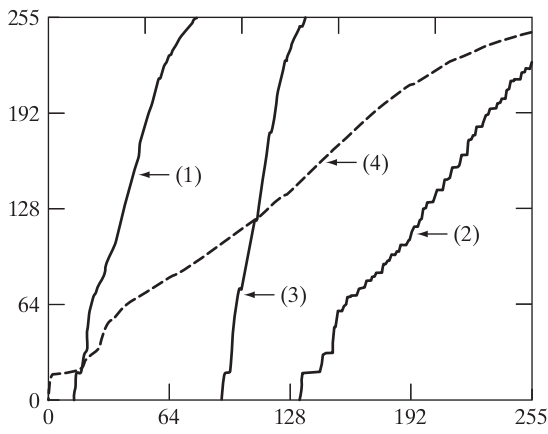
\includegraphics[width=\textwidth]{graos-3}
\caption{Transformations (1) through (4) were obtained from the histograms of the images (top-bottom) in the left column of using $s_{k} = (L-1/MN)\sum_{j=0}^{k} n_{j},\ j=0,1,\ldots,L-1$.}
\end{figure}
\end{column}
\end{columns}
\end{frame}

%----------------------------------------------------------------------------------------

\subsection{Histogram matching}

%----------------------------------------------------------------------------------------

\begin{frame}{Histogram matching}
Histogram equalization:
\begin{itemize}
\item Automatically determines a transformation function that seeks to produce an output image that has a uniform histogram.
\item If automatic enhancement is desired, this is a good approach because;
\begin{itemize}
\item the results from this technique are predictable, and;
\item the method is simple to implement.
\end{itemize}
\item However:
\end{itemize}
\begin{block}{Histogram matching}
Sometimes it is useful to be able to specify the shape of the histogram that we wish the
processed image to have.
\end{block}
\end{frame}


%----------------------------------------------------------------------------------------

\begin{frame}
\begin{figure}
\centering
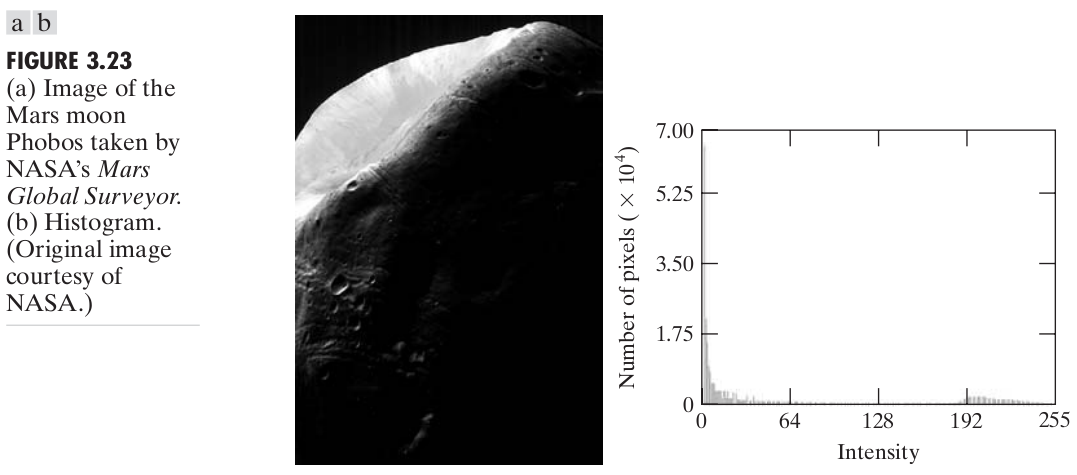
\includegraphics[width=\textwidth]{fig-3-23}
\end{figure}
\end{frame}

%----------------------------------------------------------------------------------------

\begin{frame}
\begin{columns}
\begin{column}{.5\textwidth}
\begin{figure}
\centering
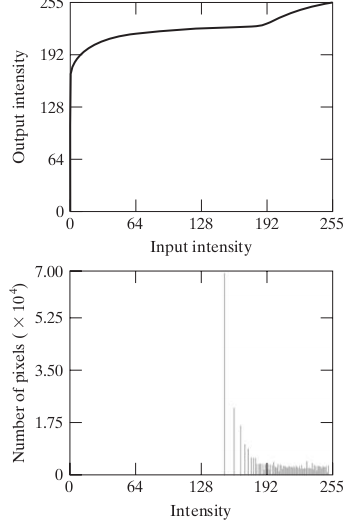
\includegraphics[width=\textwidth]{fig-3-24ab}
\end{figure}
\end{column}
\begin{column}{.5\textwidth}
\begin{figure}
\centering
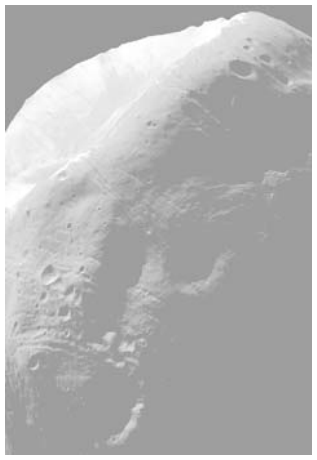
\includegraphics[width=\textwidth]{fig-3-24b}
\end{figure}
\end{column}
\end{columns}
\end{frame}

%----------------------------------------------------------------------------------------

\begin{frame}
\begin{columns}
\begin{column}{.5\textwidth}
\begin{figure}
\centering
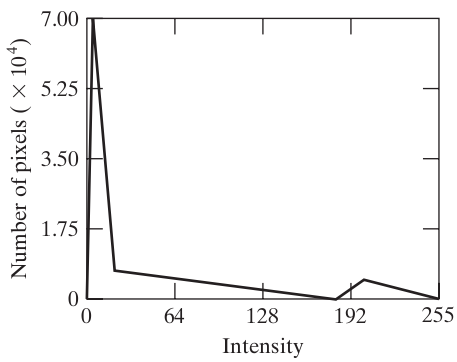
\includegraphics[width=.5\textwidth]{fig-3-25a}
\end{figure}
\begin{figure}
\centering
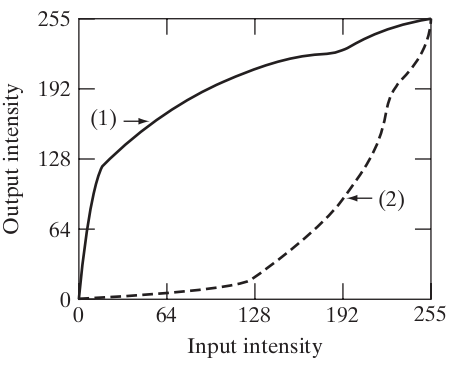
\includegraphics[width=.5\textwidth]{fig-3-25b}
\end{figure}
\begin{figure}
\centering
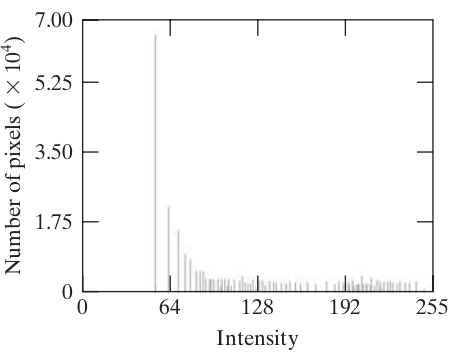
\includegraphics[width=.5\textwidth]{fig-3-25d}
\end{figure}
\end{column}
\begin{column}{.5\textwidth}
\begin{figure}
\centering
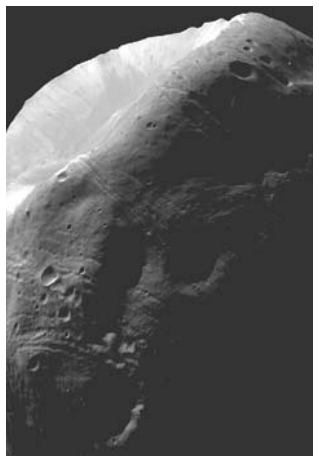
\includegraphics[width=\textwidth]{fig-3-25c}
\end{figure}
\end{column}
\end{columns}
\end{frame}

%----------------------------------------------------------------------------------------

\begin{frame}
Histogram matching is:
\begin{itemize}
\item A trial-and-error process.
\item Sometimes, the user might know what an ``average'' histogram should look like.
\item There are no general rules to specifying histograms, varying between different cases.
\end{itemize}
\end{frame}

%----------------------------------------------------------------------------------------

\subsubsection{Local histogram processing}

%----------------------------------------------------------------------------------------

\begin{frame}
\frametitle{Local histogram processing}
\begin{itemize}
\item Histogram equalization and matching are \textbf{global} techniques.
\item How to enhance details locally? Consider small windows centered on each pixel.
\item The global techniques presented can be applied locally.
\end{itemize}
\end{frame}

%----------------------------------------------------------------------------------------

\begin{frame}
\begin{figure}
\centering
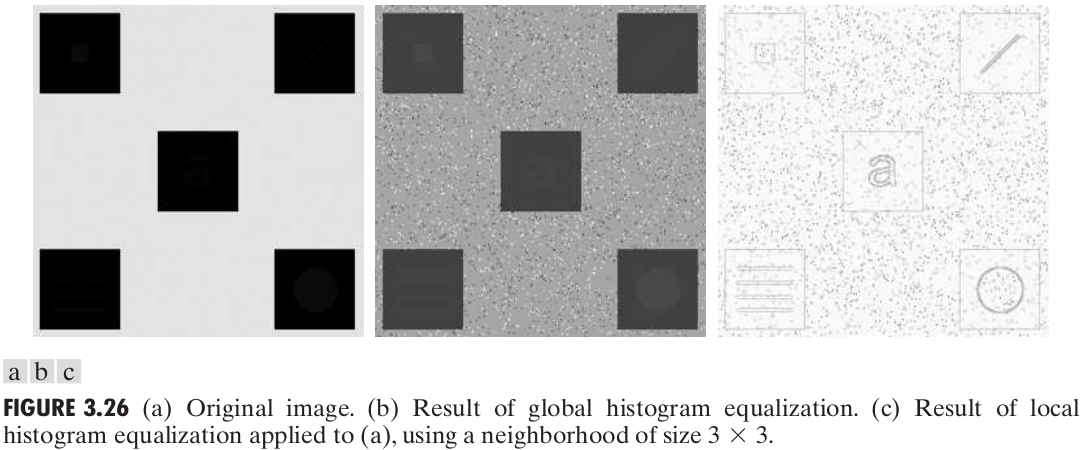
\includegraphics[width=\textwidth]{fig-3-26}
\end{figure}
\end{frame}

%----------------------------------------------------------------------------------------

\subsubsection{Using histogram statistics for image enhancement}

%----------------------------------------------------------------------------------------

\begin{frame}{Using histogram statistics for image enhancement}
Statistics obtained from an image can be used for image enhancement:
\begin{itemize}
\item $r$ denotes a discrete random variable representing intensities within range $[0,L-1]$.
\item $p(r_{i})$ denotes the normalized histogram corresponding to intensity $r_{i}$.
\item The mean
\begin{equation}
m = \sum_{i=0}^{L-1}r_{i}p(r_{i}).
\end{equation}
\item The \textit{n}th moment
\begin{equation}
\mu_{n} = \sum_{i=0}^{L-1} \left ( r_{i} - m \right )^{n} p(r_{i}).
\end{equation}
\end{itemize}
\end{frame}

%----------------------------------------------------------------------------------------

\begin{frame}
The second moment is particularly important:
\begin{equation}
\mu_{2} = \sigma^{2} = \sum_{i=0}^{L-1} \left ( r_{i} - m \right )^{2} p(r_{i}).
\end{equation}
\begin{itemize}
\item The mean $m$ is a measure of average intensity.
\item The variance $\sigma^{2}$ is a measure of contrast.
\end{itemize}
\end{frame}

%----------------------------------------------------------------------------------------

\begin{frame}
Notation when computing mean and moment on sub-images:
\begin{equation}
m_{S_{xy}} = \sum_{(s,t) \in S_{xy}} r_{s,t} p(r_{s,t}).
\end{equation}
\begin{equation}
\mu^{n}_{S_{xy}} = \sum_{(s,t)\in S_{xy}} \left ( r_{s,t} - m_{S_{xy}} \right )^{n} p\left ( r_{s,t} \right )
\end{equation}
As before, the local mean is a measure of \textbf{average intensity} in neighborhood and the local variance $\sigma^{2} = \mu^{2}$ is a measure of \textbf{intensity contrast} in that neighborhood.
\end{frame}

%----------------------------------------------------------------------------------------

\begin{frame}
\begin{columns}
\begin{column}{.5\textwidth}
Consider the SEM image of a tungsten filament.\\
We want to enhance areas which
\begin{itemize}
\item Have low intensity average \textit{wrt} the whole image.
\item Have low contrast.
\item Have not a constant contrast.
\end{itemize}
\end{column}
\begin{column}{.5\textwidth}
\begin{figure}
\centering
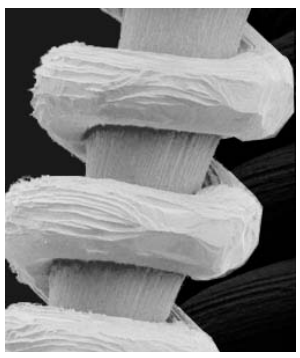
\includegraphics[width=\textwidth]{fig-3-27a}
\end{figure}
\end{column}
\end{columns}
\end{frame}

%----------------------------------------------------------------------------------------

\begin{frame}
\begin{equation}
g(x,y) = \left \{
\begin{array}{ll}
E\cdot f(x,y) & \text{if } m_{S_{xy}} \leq k_{0} m_{G} \text{ and } k_{1} \sigma_{G} \leq \sigma_{S_{xy}} \leq  k_{2} \sigma_{G} \\
f(x,y) & \text{otherwise}
\end{array}.
\right .
\label{eq:localHistProc}
\end{equation}
Where $E$ increases (or decreases) the  gray levels satisfying~(\ref{eq:localHistProc}).
\begin{figure}
\centering
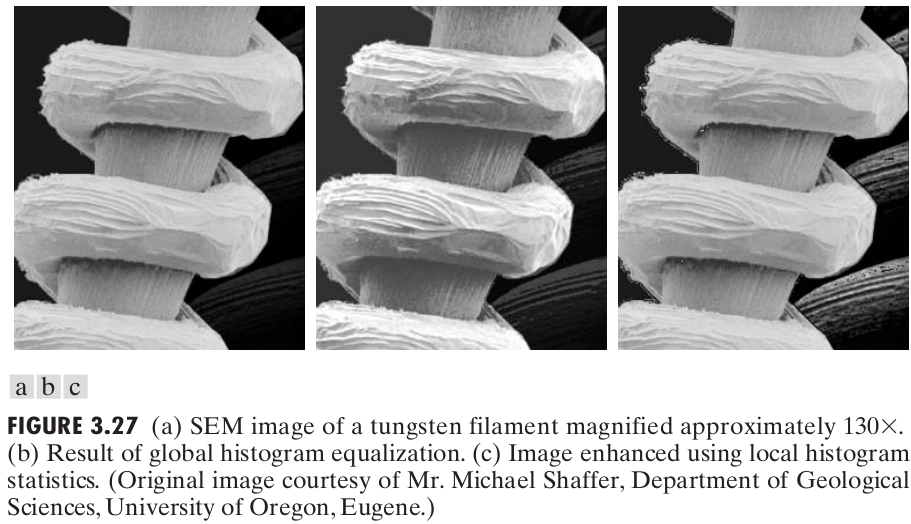
\includegraphics[width=.7\textwidth]{fig-3-27}
\end{figure}
\end{frame}

%----------------------------------------------------------------------------------------

\begin{frame}
Values (require experimentation):
\begin{itemize}
\item $E$ = 4.0. $S_{xy}$ is a $3\times 3$ region.
\item $k_{0} = 0.4,\ k_{1} = 0.02,\ k_{2}= 0.4$.
\end{itemize}
\begin{figure}
\centering
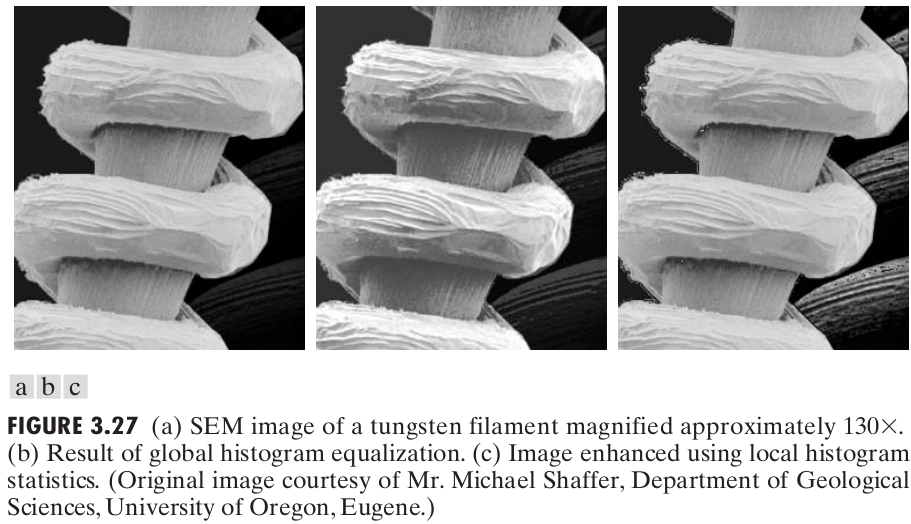
\includegraphics[width=.8\textwidth]{fig-3-27}
\end{figure}
\end{frame}

%----------------------------------------------------------------------------------------

\begin{frame}
\begin{figure}
\centering
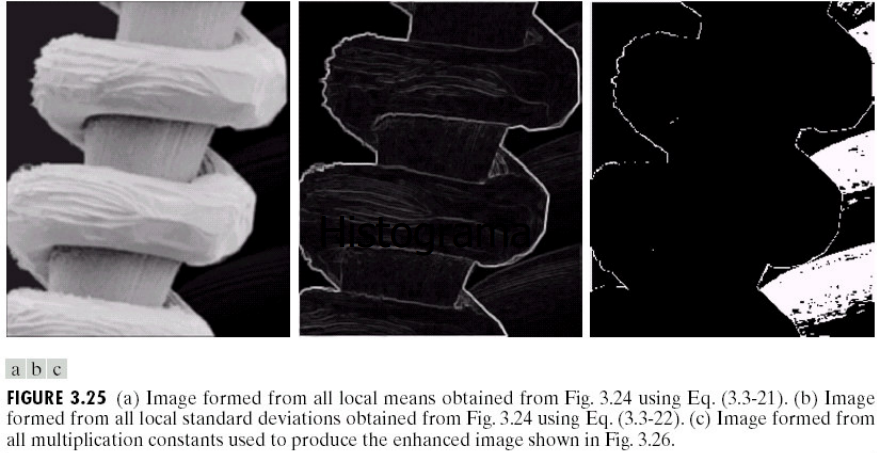
\includegraphics[width=\textwidth]{fig-3-25-old}
\end{figure}
\end{frame}

%----------------------------------------------------------------------------------------

\section{Fundamentals of spatial filtering}

%----------------------------------------------------------------------------------------

\begin{frame}
\frametitle{Spatial filtering}
\begin{itemize}
\item Spatial filtering is often used for image enhancement.
\item Term \textit{filtering} was borrowed from the frequency domain.
\item Spatial filtering can be used for non-linear filtering, which cannot be done in the frequency domain.
\end{itemize}
\end{frame}

%----------------------------------------------------------------------------------------

\subsection{The mechanics of spatial filtering}

%----------------------------------------------------------------------------------------

\begin{frame}
A spatial filter consists in
\begin{enumerate}
\item A \textit{neighborhood}.
\item A \textit{predefined operation}.
\end{enumerate}
The spatial filter can be;
\begin{itemize}
\item linear, or;
\item nonlinear.
\end{itemize}
\end{frame}

%----------------------------------------------------------------------------------------

\begin{frame}
\begin{figure}
\centering
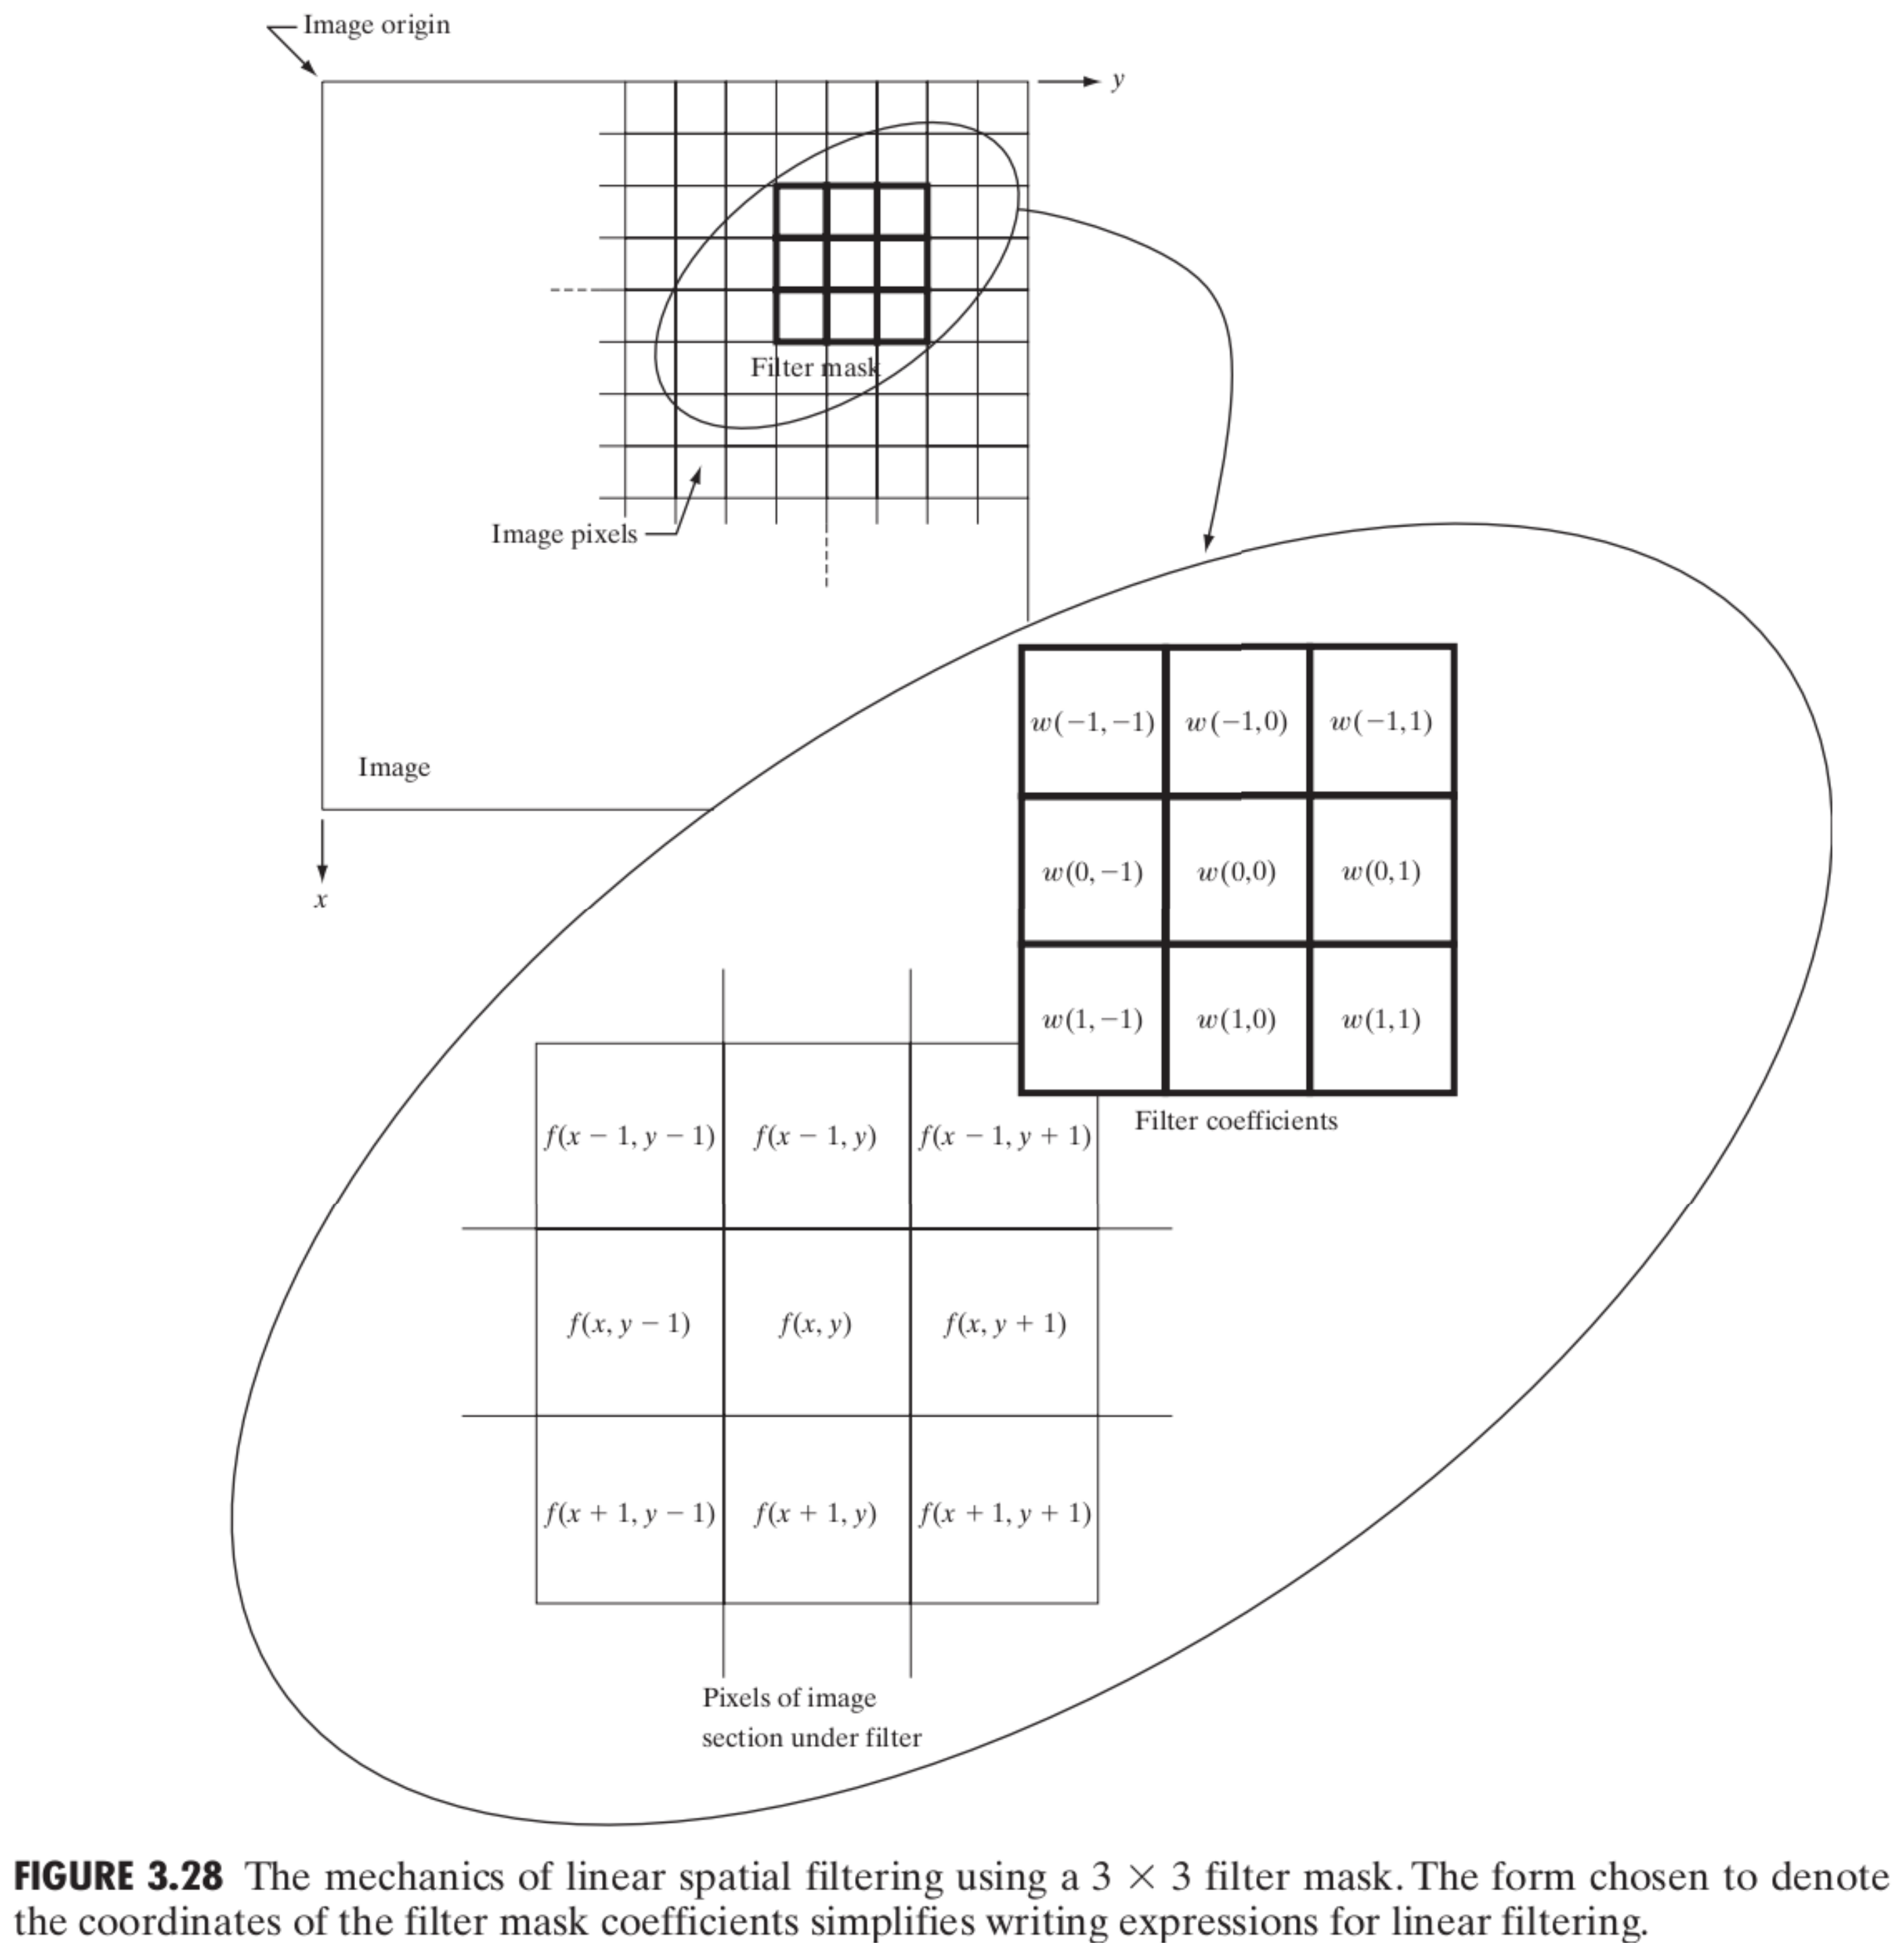
\includegraphics[width=.7\textwidth]{fig-3-28}
\end{figure}
\end{frame}

%----------------------------------------------------------------------------------------

\begin{frame}
\begin{equation}
g(x,y) = \sum_{s=-a}^{a}\sum_{t=-b}^{b} w(s,t) f(x+s, y+t),\ \ \forall\  x,y.
\end{equation}
Where:
\begin{itemize}
\item $a = (m-1)/2$ and $b=(n-1)/2$ form the window dimension $m\times n$ (both odd numbers).
\item Also called \textit{convolution}.
\item Note: the result of the operation does not change the original image.
\end{itemize}
\end{frame}

%----------------------------------------------------------------------------------------

\begin{frame}
The basic procedure consists in summing the products between the mask coefficients and the gray levels at the local image region.
\begin{columns}
\begin{column}{.5\textwidth}
\[
R = w_{1} z_{1} + w_{2} z_{2} + \ldots + w_{9} z_{9}.
\]
In general;
\[
R = w_{1} z_{1} + w_{2} z_{2} + \ldots + w_{mn} z_{mn}
\]
\[
R = \sum_{k=1}^{mn}w_{k}z_{k}
\]
\begin{equation}
R = \textbf{w}^{T} \textbf{z}
\end{equation}
\end{column}
\begin{column}{.5\textwidth}
\begin{figure}
\centering
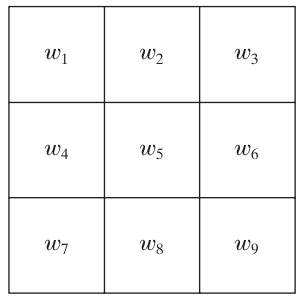
\includegraphics[width=\textwidth]{fig-3-31}
\end{figure}
\end{column}
\end{columns}
\end{frame}

%----------------------------------------------------------------------------------------

\section{Smoothing spatial filters}

%----------------------------------------------------------------------------------------

\begin{frame}
\frametitle{Smoothing filters}
\begin{itemize}
\item Smoothing filters are used for \textit{blurring} and \textit{noise reduction}.
\begin{itemize}
\item Blurring is used in pre-processing stages to remove small details for object extraction.
\item Noise reduction can be obtained also with non-linear filtering.
\end{itemize}
\item Low-pass filtering.
\begin{itemize}
\item Neighborhood average.
\item Results in a blurred image.
\end{itemize}
\end{itemize}
\end{frame}

%----------------------------------------------------------------------------------------

\subsection{Smoothing linear filters}

%----------------------------------------------------------------------------------------

\begin{frame}
Smoothing filter mask examples:
\begin{figure}
\centering
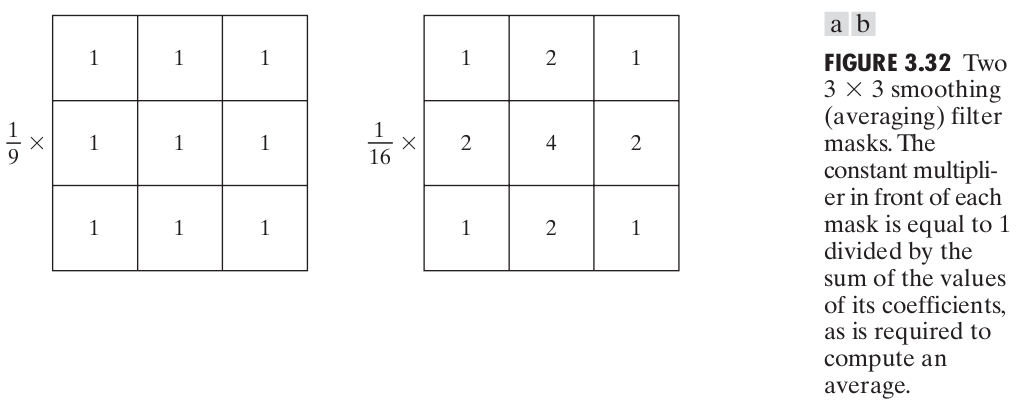
\includegraphics[width=\textwidth]{fig-3-32}
\end{figure}
\end{frame}

%----------------------------------------------------------------------------------------

\begin{frame}
\begin{columns}
\begin{column}{.5\textwidth}
Example: average filter (mask sizes = 3, 5, 9, 15, 35).\\
Notice:
\begin{itemize}
\item Blurring.
\item Blending.
\item Noise reduction.
\item Object elimination.
\item Black border.
\end{itemize}
\end{column}
\begin{column}{.5\textwidth}
\begin{figure}
\centering
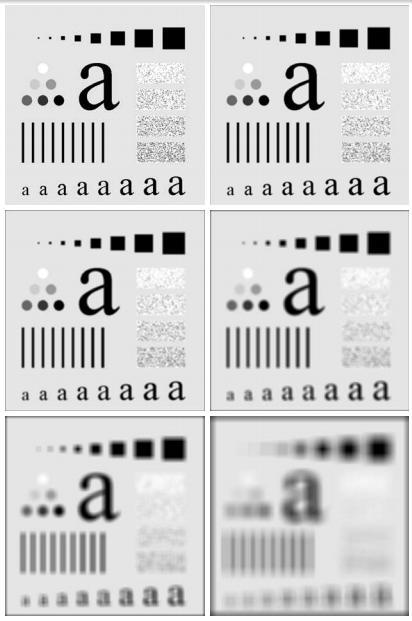
\includegraphics[width=\textwidth]{fig-3-33}
\end{figure}
\end{column}
\end{columns}
\end{frame}

%----------------------------------------------------------------------------------------

\begin{frame}
Gross representation of objects.
Note:
\begin{figure}
\centering
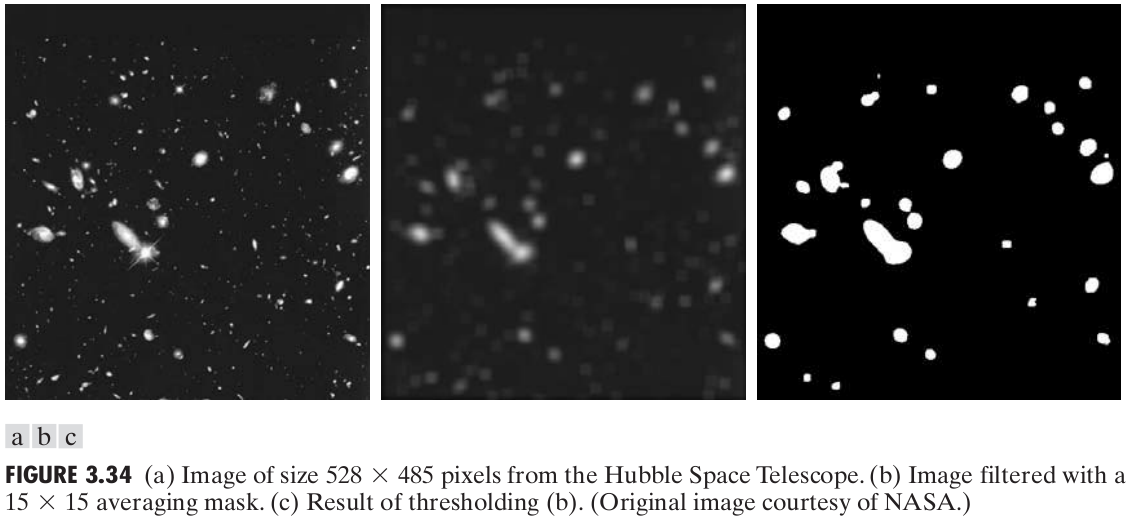
\includegraphics[width=\textwidth]{fig-3-34}
\end{figure}
\end{frame}

%----------------------------------------------------------------------------------------

\subsection{Order-statistic (non-linear filters)}

%----------------------------------------------------------------------------------------

\begin{frame}
\frametitle{Non-linear filters}
Median filter:
\begin{itemize}
\item Useful for elimination of \textit{salt-and-pepper} (or \textit{impulse}) noise.
\item The median $\xi$ of a set of values is such that half the values in the set are less than or equal to $\xi$ and half are greater than or equal to $\xi$.
\item I. e., its main function is to force points with distinct intensity levels to be more like their neighbors.
\end{itemize}
\begin{figure}
\centering
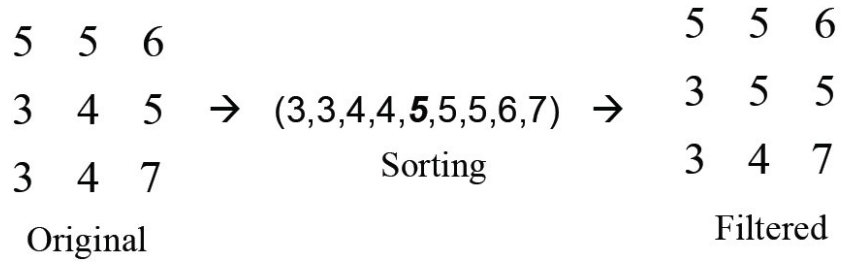
\includegraphics[width=.7\textwidth]{median-filter}
\end{figure}
\end{frame}

%----------------------------------------------------------------------------------------

\begin{frame}
Salt and pepper noise removal using the median filter:
\begin{figure}
\centering
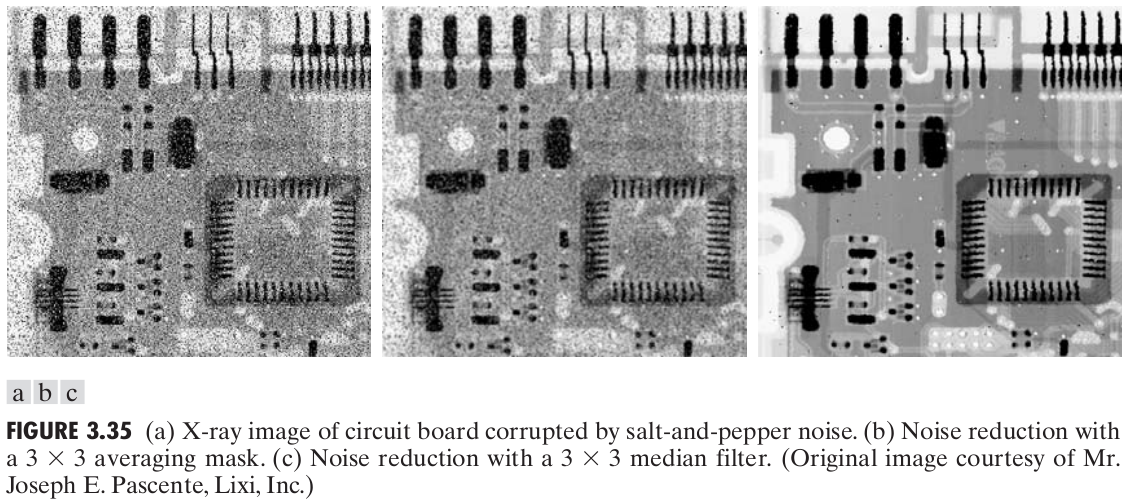
\includegraphics[width=\textwidth]{fig-3-35}
\end{figure}
\end{frame}

%----------------------------------------------------------------------------------------

\section{Sharpening spatial filters}

%----------------------------------------------------------------------------------------

\begin{frame}
\frametitle{Sharpening spatial filters}
Sharpening filters aim at:
\begin{itemize}
\item Enhancing fine details.
\item Recovering information compromised by blurring.
\end{itemize}
Applications:
\begin{itemize}
\item Electronic printing.
\item Medical imaging.
\item Industrial inspection.
\end{itemize}
\end{frame}

%----------------------------------------------------------------------------------------

\subsection{Foundation}

%----------------------------------------------------------------------------------------

\begin{frame}
In the spatial domain:
\begin{itemize}
\item Blurring (averaging) is analogous to integration.
\item Sharpening is analogous do differentiation.
\end{itemize}
\begin{block}{}
Image differentiation enhances edges and other discontinuities (e.g., noise) and deemphasizes areas with slowly varying intensities.
\end{block}
\begin{figure}
\centering
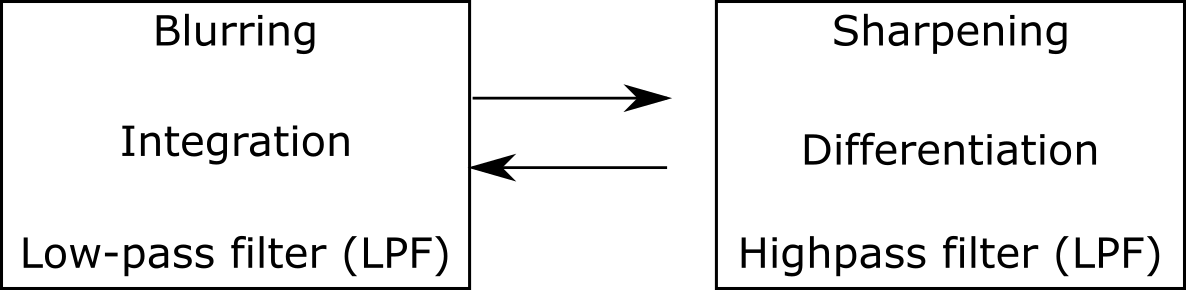
\includegraphics[width=\textwidth]{blurringVSsharpening}
\end{figure}
\end{frame}

%----------------------------------------------------------------------------------------

\begin{frame}
A first derivative:
\begin{itemize}
\item Must be zero in areas of constant intensity.
\item Must be nonzero at the onset of an intensity step or ramp.
\item Must be nonzero along ramps. 
\end{itemize}
Basic definition of a first-order derivative of a one-dimensional function:
\begin{equation}
\dfrac{\partial f}{\partial x} = f(x+1) - f(x).
\end{equation}
\end{frame}

%----------------------------------------------------------------------------------------

\begin{frame}
A second derivative:
\begin{itemize}
\item Must be zero in constant areas.
\item Must be nonzero at the onset and end of an intensity step or ramp.
\item Must be zero along ramps of constant slope.
\end{itemize}
Definition of second order derivative
\begin{equation}
\dfrac{\partial^{2} f}{\partial x^{2}} = f(x+1) + f(x-1) - 2f(x).
\end{equation}
\end{frame}

%----------------------------------------------------------------------------------------

\begin{frame}
\begin{figure}
\centering
\includegraphics[width=\textwidth]{fig-3-36}
\end{figure}
\end{frame}

%----------------------------------------------------------------------------------------

\begin{frame}
\begin{figure}
\centering
\includegraphics[width=.85\textwidth]{fig-3-38-old}
\end{figure}
\end{frame}

%----------------------------------------------------------------------------------------

\begin{frame}
Notes on derivatives:
\begin{itemize}
\item 1st derivative:
\begin{itemize}
\item Produces thicker borders.
\item Higher response to big differences (e.g., step).
\item Often used for border detection.
\end{itemize} 
\item 2nd derivative
\begin{itemize}
\item More sensitive to finer details.
\item Better for image enhancement, since its more sensitive.
\item Produces double response to step.
\end{itemize}
\end{itemize}
\end{frame}

%----------------------------------------------------------------------------------------

\subsection{Second derivative - The Laplacian}

%----------------------------------------------------------------------------------------

\begin{frame}
Simplest \textit{isotropic}\footnote{Independent of orientation} derivative operator: The Laplacian:
\begin{equation}
\nabla^{2}f = \dfrac{\partial^{2} f}{\partial x^{2}} + \dfrac{\partial^{2}f}{\partial y^{2}}.
\end{equation}
Since:
\[
\dfrac{\partial^{2} f}{\partial x^{2}} = f(x+1) + f(x-1) - 2f(x)
\]
and
\[
\dfrac{\partial^{2} f}{\partial y^{2}} = f(y+1) + f(y-1) - 2f(y).
\]
We have
\begin{equation}
\boxed{\nabla^{2}f = f(x+1,y) + f(x-1,y) + f(x, y+1) + f(x,y-1) -4f(x,y)}.
\end{equation}
\end{frame}

%----------------------------------------------------------------------------------------

\begin{frame}
\[
\boxed{\nabla^{2}f = f(x+1,y) + f(x-1,y) + f(x, y+1) + f(x,y-1) -4f(x,y)}
\]
\begin{figure}
\centering
\includegraphics[width=.7\textwidth]{fig-3-37}
\end{figure}
\end{frame}

%----------------------------------------------------------------------------------------

\begin{frame}
Because the Laplacian is a derivative operator: 
\begin{itemize}
\item It highlights intensity
discontinuities in an image.
\item De-emphasizes regions with slowly varying intensity levels.
\end{itemize}
The basic way to use the Laplacian for image sharpening is:
\begin{equation}
\boxed{
g(x,y) =  f(x,y) + c \nabla^{2} f(x,y)
}
\end{equation}
where:
\begin{itemize}
\item $f(x,y)$ and $g(x,y)$ are the input and sharpened images.
\item $c$ is $-1$ or $+1$ if the center of the filter is negative or positive, respectively.
\end{itemize}
\end{frame}

%----------------------------------------------------------------------------------------

\begin{frame}
\begin{columns}
\begin{column}{.5\textwidth}
\begin{figure}
\centering
\includegraphics[width=.4\textwidth]{fig-3-38a}
\end{figure}
\begin{figure}
\centering
\includegraphics[width=\textwidth]{fig-3-38bc}
\end{figure}
\end{column}
\begin{column}{.5\textwidth}
\begin{figure}
\centering
\includegraphics[width=\textwidth]{fig-3-38de}
\end{figure}
\begin{figure}
\centering
\includegraphics[width=.25\textwidth]{fig-3-38leg}
\end{figure}
\end{column}
\end{columns}
\end{frame}

%----------------------------------------------------------------------------------------

\subsection{High-boost filtering}

%----------------------------------------------------------------------------------------

\begin{frame}
\frametitle{High-boost\footnote{``Alto reforço''} filtering}
\begin{enumerate}
\item Blur the original image.
\item Subtract the blurred image from the original (the resulting difference is called the \textit{mask}).
\item Add the mask to the original.
\end{enumerate}
\end{frame}

%----------------------------------------------------------------------------------------

\begin{frame}
More formally:
\[
g_{mask} = f(x,y) - \underbrace{\overline{f}(x,y)}_{\text{Blurred image}}
\]
\begin{equation}
g(x,y) = f(x,y) + k \cdot g_{mask} (x,y).
\end{equation}
Where:
\begin{itemize}
\item $k\geq 0$.
\item $k=1$, we have unsharp masking.
\item When $k>1$ we have \textit{highboost filtering}.
\end{itemize}
\end{frame}

%----------------------------------------------------------------------------------------

\begin{frame}
\begin{figure}
\centering
\includegraphics[width=\textwidth]{fig-3-39}
\end{figure}
\end{frame}

%----------------------------------------------------------------------------------------

\begin{frame}
\begin{columns}
\begin{column}{.25\textwidth}
\begin{figure}
\centering
\includegraphics[width=\textwidth]{fig-3-40}
\end{figure}
\end{column}
\begin{column}{.15\textwidth}
\begin{figure}
\centering
\includegraphics[width=\textwidth]{fig-3-40leg}
\end{figure}
\end{column}
\end{columns}
Note: In fig 3.40 (d) and (e), k=1 and 4.5.
\end{frame}

%----------------------------------------------------------------------------------------

\begin{frame}
Examples with $k=$1.1, 1.15 and 1.2.
\begin{figure}
\centering
\includegraphics[width=.7\textwidth]{high-boost-filtering}
\end{figure}
\end{frame}

%----------------------------------------------------------------------------------------

\subsection{First-Order Derivatives for (Nonlinear) Image Sharpening -- The Gradient}

%----------------------------------------------------------------------------------------

\begin{frame}
The gradient of $f(x,y)$ is defined 	as the two dimensional column vector:
\begin{equation}
\nabla f \equiv \left (
\begin{array}{c}
g_{x}\\
g_{y}
\end{array}
\right ) =
\left (
\begin{array}{c}
\dfrac{\partial f}{\partial x}\\
\dfrac{\partial f}{\partial y}
\end{array}
\right )
\end{equation}
This vector points in the direction of the greatest rate of change of $f$ at $(x, y)$.\\
The \textit{magnitude} of vector $\nabla f$ is
\begin{equation}
M(x,y) = mag(\nabla f) = \sqrt{g_{x}^{2} + g_{y}^{2}}.
\end{equation}
is the value at $(x, y)$ of the rate of change in the direction of the gradient vector.
\end{frame}

%----------------------------------------------------------------------------------------

\begin{frame}
Note that $M(x, y)$ is an image of the same size as the original.\\
In some implementations, it is more suitable computationally to approximate the squares and square root operations by absolute values:
\begin{equation}
M(x,y) \approx |g_{x}| + |g_{y}|.
\end{equation}
\end{frame}

%----------------------------------------------------------------------------------------

\begin{frame}
Now we define discrete approximations to the preceding equations and formulate the masks.
\begin{itemize}
\item The smallest filter masks are of
size $3\times 3$.
\end{itemize}
\begin{figure}
\centering
\includegraphics[width=.4\textwidth]{fig-3-41a}
\end{figure}
\end{frame}

%----------------------------------------------------------------------------------------

\begin{frame}
Approximations to $g_{x}$ and $g_{y}$ using a $3\times 3$ neighborhood centered on $z_{5}$ are as follows (The \textit{Sobel} operators):
\begin{equation}
g_{x} = \dfrac{\partial f}{\partial x} = (z_{7} + 2z_{8} + z_{9} ) - (z_{1} + 2z_{2} + z_{3} )
\end{equation}
and
\begin{equation}
g_{y} = \dfrac{\partial f}{\partial y} = (z_{3} + 2z_{6} + z_{9} ) - (z_{1} + 2z_{4} + z_{7} )
\end{equation}
\begin{figure}
\centering
\includegraphics[width=.4\textwidth]{fig-3-41a}
\end{figure}
\end{frame}

%----------------------------------------------------------------------------------------

\begin{frame}
The \textit{Sobel} operators:
\begin{figure}
\centering
\includegraphics[width=.4\textwidth]{fig-3-14-d-e}
\end{figure}
Notes:
\begin{itemize}
\item The weight of $2$ in the center coefficient is to achieve some smoothing by giving more importance to the center point.
\item The magnitude of the gradient is obtained with:
\begin{equation}
M(x,y) \approx |g_{x}| + |g_{y}|.
\end{equation}
\end{itemize}
\end{frame}

%----------------------------------------------------------------------------------------

\begin{frame}
\begin{block}{Note}
The coefficients in all masks sum to 0 (null response in an area of constant intensity).
\end{block}
\end{frame}

%----------------------------------------------------------------------------------------

\begin{frame}
Application: Industrial inspection.
\begin{itemize}
\item Aid humans.
\item Automatic detection.
\end{itemize}
\begin{figure}
\centering
\includegraphics[width=\textwidth]{fig-3-42}
\end{figure}
\end{frame}

%----------------------------------------------------------------------------------------

\section{Combining spatial enhancement methods}

%----------------------------------------------------------------------------------------

\begin{frame}
\begin{columns}
\begin{column}{.5\textwidth}
Example: Sharpening an image of nuclear whole body bone scan (detect bone infection and tumors).\\
Observe:
\begin{itemize}
\item Narrow dynamic range.
\item High noise.
\end{itemize}
Strategy:
\begin{enumerate}
\item Laplacian to enhance detail.
\item Gradient to enhance borders.
\end{enumerate}
\end{column}
\begin{column}{.5\textwidth}
\begin{figure}
\centering
\includegraphics[width=.8\textwidth]{Fig0343(a)(skeleton_orig).jpg}
\end{figure}
\end{column}
\end{columns}
\end{frame}

%----------------------------------------------------------------------------------------

\begin{frame}
\begin{columns}
\begin{column}{.3\textwidth}
\begin{figure}
\centering
\includegraphics[width=\textwidth]{Fig0343(a)(skeleton_orig).jpg}
\caption{$f(x,y)$}
\end{figure}
\end{column}
\begin{column}{.3\textwidth}
\begin{figure}
\centering
\includegraphics[width=\textwidth]{fig-3-43-b}
\caption{$\nabla^{2} f(x,y)$ (scaled).}
\end{figure}
\end{column}
\begin{column}{.3\textwidth}
\begin{figure}
\centering
\includegraphics[width=\textwidth]{fig-3-43-c}
\caption{$g(x,y) = f(x,y) - c\nabla^{2} f(x,y)$}
\end{figure}
\end{column}
\end{columns}
\end{frame}

%----------------------------------------------------------------------------------------

\begin{frame}
The Laplacian:
\begin{itemize}
\item Second-order derivative operator capable of enhancing fine details.
\item Noisy.
\end{itemize}
\end{frame}

%----------------------------------------------------------------------------------------

\begin{frame}
\begin{columns}
\begin{column}{.5\textwidth}
\begin{figure}
\centering
\includegraphics[width=.7\textwidth]{Fig0343(a)(skeleton_orig).jpg}
\caption{$f(x,y)$}
\end{figure}
\end{column}
\begin{column}{.5\textwidth}
\begin{figure}
\centering
\includegraphics[width=.7\textwidth]{fig-3-43-d}
\caption{$M(x,y) = |g_{x}| + |g_{y}|$.}
\end{figure}
\end{column}
\end{columns}
\end{frame}

%----------------------------------------------------------------------------------------

\begin{frame}
The gradient:
\begin{itemize}
\item Stronger average response in areas of significant image transition (ramps and steps).
\item Lower response to noise and fine detail.
\end{itemize}
\end{frame}

%----------------------------------------------------------------------------------------

\begin{frame}
\begin{figure}
\centering
\includegraphics[width=\textwidth]{filter-combination}
\end{figure}
\end{frame}

%----------------------------------------------------------------------------------------

%\begin{frame}
%\begin{figure}
%\centering
%\includegraphics[width=1.1\textwidth]{result1}
%\end{figure}
%\end{frame}

%----------------------------------------------------------------------------------------

\begin{frame}
Conclusions:
\begin{itemize}
\item Processes can be linked to achieve results better than single techniques.
\item Strategy depends on the application.
\end{itemize}
Applications
\begin{itemize}
\item Radiology.
\item Physicians are unlikely to derive diagnosis from enhanced images, but they serve as clues for further investigations.
\end{itemize}
\end{frame}

%----------------------------------------------------------------------------------------

\begin{frame}
Areas where the enhanced images are used:
\begin{itemize}
\item Printing industry.
\item Image-based product inspection.
\item Forensics.
\item Microscopy.
\item Surveillance.
\end{itemize}
\end{frame}


%----------------------------------------------------------------------------------------

\section{Fuzzy logic for intensity transf. and filtering}

%----------------------------------------------------------------------------------------

\begin{frame}
Application of fuzzy sets to:
\begin{itemize}
\item Intensity transformation.
\item Spatial filtering.
\end{itemize}
Definitions:
\begin{itemize}
\item A \textit{set} is a collection of elements.
\item \textit{Set theory} conveys tools dealing with operations \textbf{on} and \textbf{among} sets.
\item \textit{Crispy} set membership: an element \textbf{is} or \textbf{isn't} inside a set.
\end{itemize}
\end{frame}

%----------------------------------------------------------------------------------------

\begin{frame}
Example:
\begin{itemize}
\item $Z =$ set of all people.
\item $A = $ subset of young people.
\item Suppose \textit{threshold} = 20 years.
\item Someone 20 years (and 1 second) old?!
\end{itemize}
\begin{figure}
\centering
\includegraphics[width=\textwidth]{fig-3-44}
\end{figure}
\end{frame}

%----------------------------------------------------------------------------------------

\begin{frame}
A person now can be:
\begin{itemize}
\item Young.
\item Relatively young.
\item 50\% young.
\item Not so young.
\item Not young, etc.
\end{itemize}
\end{frame}

%----------------------------------------------------------------------------------------

\begin{frame}
\begin{block}{Fuzzy}
Infinite valued membership functions;
\begin{itemize}
\item are the foundation of \textit{fuzzy logic}, and;
\item the sets generating them may be viewed as \textit{fuzzy sets}.
\end{itemize}
\end{block}
\end{frame}

%----------------------------------------------------------------------------------------

\subsection{Principles of Fuzzy set theory}

%----------------------------------------------------------------------------------------

\begin{frame}
Define:
\begin{itemize}
\item $Z$ = set of elements.
\item $z$ = generic element of $Z$; $Z=\{z\}$.
\end{itemize}
\begin{block}{Definition}
A \textit{fuzzy set} in $Z$ is characterized by a membership function $\mu_{A}(z)$, that associates with each element of $Z$ a real number in the interval $[0,1]$.
\end{block}
\begin{figure}
\centering
\includegraphics[width=.8\textwidth]{fig-3-44}
\end{figure}
\end{frame}


\begin{frame}
\begin{itemize}
\item The value of $\mu_{A}(z)$ represents the \underline{grade of membership} of $z$ in $A$.
\end{itemize}
An element $z$ is;
\begin{itemize}
\item A \underline{full member} of $A$ if $\mu_{A}(z)=1$.
\item \underline{Not a member} of $A$ if $\mu_{A}(z)=0$.
\item A \underline{partial member} of $A$ if $0<\mu_{A}(z)<1$.
\end{itemize}
\begin{itemize}
\item Crispy sets are a particular case of Fuzzy sets.
\end{itemize}
\end{frame}

%----------------------------------------------------------------------------------------

\begin{frame}
Basic definitions:
\begin{itemize}
\item \textbf{Empty set}: A fuzzy set is \textit{empty} if and only if its membership function is identically zero in $Z$.
\item \textbf{Equality}: Two fuzzy sets $A$ and $B$ are equal, written $A = B$, if and only if $\mu_{A} (z) = \mu_{B}(z)$ for all $z \in Z$.
\item \textbf{Complement}: The \textit{complement} (NOT) of a fuzzy set $A$, denoted by $\bar{A}$, or NOT($A$), is defined as the set whose membership function is
\[
\mu_{\bar{A}}(z) = 1 - \mu_{A}(z),\ \ \forall z \in Z.
\]
\end{itemize}
\end{frame}

%----------------------------------------------------------------------------------------

\begin{frame}
Basic definitions:
\begin{itemize}
\item \textbf{Subset}: A fuzzy set $A$ is a subset of a fuzzy set $B$ if and only if
\[
\mu_{A} (z) \leq \mu_{B}(z),\ \ \forall z \in Z.
\]
\item \textbf{Union}: The \textit{union} (OR) of two fuzzy sets $A$ and $B$, denoted $A \cup B$, or $A$~OR~$B$, is a fuzzy set $U$ with membership function
\[
\mu_{U}(z) = \max \left [ \mu_{A}(z), \mu_{B}(z) \right ],\ \ \forall z \in Z.
\]
\end{itemize}
\end{frame}

\begin{frame}
Basic definitions:
\begin{itemize}
\item \textbf{Intersection}: The intersection (AND) of two fuzzy sets $A$ and $B$, denoted, $A \cap B$ or $A$ AND $B$, is a fuzzy set $I$ with membership function
\[
\mu_{U}(z) = \min \left [ \mu_{A}(z), \mu_{B}(z) \right ],\ \ \forall z \in Z.
\]
\end{itemize}
\end{frame}

%----------------------------------------------------------------------------------------

\begin{frame}
\begin{figure}[!h]
\centering
\includegraphics[width=\textwidth]{fig-3-45}
\end{figure}
\end{frame}

%----------------------------------------------------------------------------------------

\subsection{Membership functions}

%----------------------------------------------------------------------------------------

\begin{frame}
\begin{figure}[!h]
\centering
\includegraphics[width=\textwidth]{table-3-6}
\end{figure}
\end{frame}

%----------------------------------------------------------------------------------------

\begin{frame}
\begin{figure}[!h]
\centering
\includegraphics[width=\textwidth]{table-3-6-2}
\end{figure}
\end{frame}

%----------------------------------------------------------------------------------------

\subsection{Using Fuzzy sets}

%----------------------------------------------------------------------------------------

\begin{frame}
\begin{figure}
\includegraphics[width=.7\textwidth]{fuzzy1.png}
\end{figure}
\begin{figure}
\includegraphics[width=.7\textwidth]{fuzzy2.png}
\end{figure}
\end{frame}

%\begin{frame}
%categorize a given type of
%fruit into three groups:
%\begin{enumerate}
%\item Verdant.
%\item Half-mature.
%\item Mature.
%\end{enumerate}
%\end{frame}

%----------------------------------------------------------------------------------------

\end{document}

%----------------------------------------------------------------------------------------
